%Oldaltorest is alkalmazhatunk
% \pagebreak
%laptores:
% \newpage


\documentclass[12pt]{report}
\usepackage[utf8]{inputenc}
%\usepackage[latin2]{inputenc}% ekezetes szavak bevitelehez
\usepackage[T1]{fontenc}
\def\magyarOptions{defaults=hu-min}
\usepackage[magyar]{babel}

\usepackage{times}
\usepackage{tcolorbox}

\usepackage{amsmath}
\usepackage{amssymb}
\usepackage{amsthm}

\usepackage{fancyhdr}

\usepackage{graphicx}
\usepackage{psfrag}

\usepackage{setspace}

\graphicspath{ {./images/} }

%Margok:
\hoffset -1in
\voffset -1in
\oddsidemargin 35mm
\textwidth 150mm
\topmargin 15mm
\headheight 10mm
\headsep 5mm
\textheight 237mm

% \onehalfspacing
\linespread{1.25}

\begin{document}


\thispagestyle{empty}

\begin{center}
{\Large\bf Szegedi Tudományegyetem}

\vspace{0.5cm}

{\Large\bf Informatikai Intézet}

\vspace*{8.5cm}


{\Huge\bf SZAKDOLGOZAT}


\vspace*{7cm}

{\LARGE\bf Marosi Márk Dániel}

\vspace*{0.6cm}

{\Large\bf 2022}

\end{center}

\newpage


\fancypagestyle{plain}{
\fancyhf{}
\fancyfoot[R]{\thepage}
\renewcommand{\headrulewidth}{0pt}
}


\pagestyle{fancy}
\fancyhf{}
\fancyhead[L]{Domain specifikus szöveg feldolgozása kép alapú dokumentumokon}
\fancyfoot[R]{\thepage}


\thispagestyle{empty}

\begin{center}
\vspace*{1cm}
{\Large\bf Szegedi Tudományegyetem}

\vspace{0.5cm}

{\Large\bf Informatikai Intézet}

\vspace*{3.8cm}


{\LARGE\bf Domain specifikus szöveg feldolgozása kép alapú dokumentumokon}


\vspace*{3.5cm}

{\Large Diplomamunka}

\vspace*{4cm}

{\large
\begin{tabular}{c@{\hspace{4cm}}c}
\emph{Készítette:}     &\emph{Témavezető:}\\
\textbf{Marosi Márk Dániel}  &\textbf{Janurik Viktor Bálint}\\
Gazdaságinformatika szakos     &Tanszéki mérnök\\
hallgató&
\end{tabular}
}

\vspace*{2cm}

{\Large
Szeged
\\
\vspace{2mm}
2022
}
\end{center}

\renewcommand{\contentsname}{Tartalomjegyzék}

\chapter*{Feladatkiírás}
\addcontentsline{toc}{section}{Feladatkiírás}

A digitalizáció és az automatizáció terjedésével egyre nagyobb az igény olyan programokra, melyek kép alapú dokumentumokról beolvasott szöveget képesek domain függően feldolgozni és osztályozni predikciók, szövegkörnyezet és a dokumentumon elfoglalt pozíció alapján.
A szakdolgozat célja egy ilyen program elkészítése egy tetszőlegesen választott domainnel.


\chapter*{Tartalmi összefoglaló}
\addcontentsline{toc}{section}{Tartalmi összefoglaló}

A szakdolgozat a kép alapú dokumentumok domain specifikus szövegfeldolgozásáról szól, ahol a kiválasztott domain a személyi igazolvány lett. Az adatvédelmi problémák elkerülése okán magam által szerkesztett, egyéni kinézettel készült személyi igazolványokat mutatok be és használok fel a szakdolgozatban.
A szakdolgozat bemutatja azokat az alkalmazásokat, melyek már bárki számára elérhetőek, rávilágít ezek hiányosságaira, majd végigkíséri az olvasót egy olyan alkalmazás fejlesztésében, mely ezeket a hiányosságokat próbálja pótolni.
A projekt megvalósítása a legújabb, ingyenesen elérhető programcsomagok és függvénykönyvtárak (EasyOCR, OpenCV) segítségével, valamint egy saját kulcs-érték párokat felismerő algoritmussal, Pyhton programozási nyelvben történt.
A fejlesztés végeredménye egy olyan asztali alkalmazás, mely a bemenetként adott kép alapú személyi igazolványról képes a szöveget kinyerni, az összetartozó adatokat párokba rendezni, majd ezt egy csv kitejesztésű fájlba exportálni. \\

\noindent
Kulcsszavak: szövegfeldolgozás, szövegkinyerés, képfeldolgozás, dokumentum

% \begin{itemize}

    % \item Téma megnevezése:
    % Domain specifikus szöveg feldolgozása kép alapú dokumentumokon

    % \item Feladat megfogalmazása:
    % A szakdolgozat témája és célja az Informatikai Intézet Cisco laborjának távoli elérés rendszerének korszerűsítési keretében történő további két modul fejlesztése.

    % \item A teljes projekt modulokra bontása, munkamegosztás:
    % Egy ilyen projekt túl nagy feladat lett volna egyetlen hallgató számára, éppen ezért a három modult -- web-es frontend, konzolos backend, es az ellenőrző/naplózó köztes modul -- három szakdolgozó fejleszti.

    % \item Alkalmazott módszerek:
    % \begin{itemize}
        % \item Python: A teljes projekt Python nyelven készült, kiegészítve több library-vel: MySQL connector, Pika, Netmiko stb.
        % \item MySQL: a rendszer backend-jéül egy mysql 8.0 szerver szolgál
        % \item RabbitMQ: a komponensek közötti kommunikáció a Rabbit Message Queue segítségével lett megvalósítva
    % \end{itemize}

    % \item Eredmények:
    % A fejlesztés produktuma egy, már alapjaiban működő rendszer, ami további tesztelések, és az ott előjövő problémák javításai után készen áll arra, hogy átvegye a jelenlegi rendszer feladatát.

% \end{itemize}

\tableofcontents

\chapter*{Bevezetés}
\addcontentsline{toc}{section}{Bevezetés}
A témaválaszatásomat az informatikai rendszerek elképesztő gyorsaságú fejlődésének gondolata alapozta meg. Egy olyan világban élünk, ahol az okos eszközök elkezdték kiváltani a manuális munkavégzési folyamatokat, vagy azokat egyszerűbbé tették. Minden nap a zsebünkben hordunk egy olyan kompakt eszközt, amely rendelkezik kamerával. Az okostelefonok kamerája, és egy erre fejlesztett applikáció együtt képes kiváltani egy hagyományos szkenner hardvert.

Ezen túlmenve, egyes felsőbb kategóriás telefonok már képesek fényképről felismerni szöveget, és opciót biztosítanak a szöveg kinyerésére is. Amennyiben előttünk van egy névjegykártya, és szeretnénk róla egy nevet vagy telefonszámot gyorsan kimásolni anélkül, hogy nekünk kelljen manuálisan begépelni, egyszerűen készítenünk kell róla egy fényképet, és amennyiben a telefon szöveget talál a képen, azt kimásolhatóvá és vágólapra illeszthetővé teszi a felhasználó számára, ezzel értékes időt spórova, továbbá a hibázás lehetőségét is csökkentve.
Mivel ezek a szoftverek egyre elterjedtebbek, szerettem volna mélyebben belelátni ebbe a témába, és egy nemrég történt tapasztalat csak felerősítette szakmai érdeklődésem a szövegfelismerés és feldolgozás kapcsán. 

Egy határátkelésnél történt, hogy a személyi igazolványomat egy kis méterű, kompakt szkennelőgépbe helyezték, és néhány másodperc alatt minden adatom, ami a személyi igazolványomon volt, a határrendészet szoftverébe került. Ez a folyamat egy olyan plusz lépést tartalmaz az előző, okostelefonos példához képest, hogy itt nem csak az igazolványon található szöveg került felismerésre és beolvasásra, mint egy nagy adathalmaz, hanem a szoftver képes volt ezt az adathalmazt megfelelően szétbontani és osztályozni, felismerte hogy melyik adat a név, melyik adat az állampolgárság, és így tovább.

A szakdolgozatom készítése során a célom, hogy ezt a témát körbejárjam, felkutassam a legújabb technológiákat, és elkészítsek egy programot, mely lehetővé teszi a hatékony szövegfeldolgozást.
% Ennek megfelelően szakdolgozatom tartalmát négy fő részre tagoltam. A dolgozat első részében a jelenleg bárki számára elérhető szövegfelismerő rendszerek közül bemutatok néhányat, majd rávilágítok azok hiányosságaira. A második részben a jelenleg legismertebb és legmodernebb technológiák utáni kutatásom eredményét fogom részletezni, mélyebben kifejteni azt, hogyan működnek azok a hasonló felhasználási célú redszerek, melyeket jelenleg az iparban használnak. A harmadik részben ismertetem és összehasonlítom azokat a keretrendszereket, amelyeket érdemes lehet felhasználni a projektemben, továbbá a teljes implementáció és fejlesztési folyamat bemutatásra kerül lépésről lépésre. A negyedik részben az elkészült program használatát, komponenseit és felépítését fogom ismertetni.


% \begin{figure}[h]
    % \centering
    % \includegraphics[scale=0.3]{topology.eps}
    % \caption{A Cisco labor izolált topológiája}
% \end{figure}

\chapter{Jelenlegi rendszerek}
\section{Jelenlegi rendszerek bemutatása}

Manapság egy átlagos felhasználónak képről történő szövegkinyerésre telefonos vagy web alapú applikációk segítségével van lehetősége. Ez a legegyszerűbb módszer, mert könnyen kezelhető, nem igényel hozzáértést, ingyenesen igénybe vehető, gyors és megbízható. A következőkben egy általam készített, nem valós adatokat tartalmazó minta igazolványon fogom tesztelni az egyik applikációt. \cite{onlineocr}

\newline

\begin{figure}[h]
  \centerline{\includegraphics[scale=.25]{example_id_card_1.eps}}
  \caption{minta igazolvány}
\end{figure}

\pagebreak

A weboldalon található egy fájl feltöltésre alkalmas mező, ide kell tallózni a képet, melyről szeretnénk kinyerni a szöveget, ezután pedig el kell indítani a beolvasási folyamatot, mely körülbelül 5 másodpercet vesz igénybe. A folyamat végén egy szövegmezőből kimásolhatóvá válik a képről kinyert szöveg. A webapplikáció az előbb bemutatott képről az alábbi szöveghalmazt nyerte ki:
\newline
\begin{tcolorbox}
    IDENTIFICATION CARD Family name and Given name: MAROSI MARK DANIEL Sex: MALE Nationality: Date of birth: Date of expiry: Document number: CAN: 123456 HUN 21/09/1999 04/11/2023 123456AB
\end{tcolorbox}
\newline
\noindent
Az eredményt megvizsgálva megállapítható, hogy a képből kinyert szöveg hibátlan, a betű és a szám alapú adatok is helyesen jelennek meg. Viszont azt is észrevehetjük, hogy az adatok rendezetlenek, kézi korrigálást igényelne, hogy az összetartozó szövegek egymás mellé kerüljenek.

\section{Jelenlegi rendszerek hiányosságai}

Tegyük fel, hogy egy olyan szituációban találjuk magunkat, ahol több személyi igazolványt kell digitalizálnunk, például egy Excel táblázatban eltárolni a kártyán olvasható adatokat. Erre három esetet fogok felvázolni. Az első a klasszikus módszer, ahol közvetlenül a személyi igazolványról írjuk át az adatokat a táblázatba, kézzel begépelve. A második módszer az előbbiekben bemutatott webapplikáció segítségével történne, a harmadik eset pedig egy olyan program használatát feltételezi, melyet a szakdolgozatom keretében szeretnék elkészíteni.

Amennyiben az első, klasszikus módszert választjuk, kézzel kell beírnunk minden egyes adatot, betűről betűre, számról számra. A három módszer közül ez a leghosszabb és legtöbb emberi hibalehetőséget rejtő módszer. Hibázhatunk az adatok olvasásánál, hibázhatunk az adatok begépelése során, valamint ott is hibázhatunk, hogy nem jó cellába visszük fel az értékeket, elcsúszunk valahol.

A második módszer az első módszerben felvázolt három hibalehetőségből kettőt minimálisra csökkent, ezek a beolvasási és begépelési hibák. A beolvasást egy olyan technológiára alapozva végzi a szoftver, amit a szakdolgozat következő fejezeteiben fogok részletesebben bemutatni. Fontos megjegyezni, hogy egyes weboldalak lehetőséget biztosítanak egyszerre akár több kép feltöltésére, ezzel is gyorsítva a folyamatot. A képről történő szövegkinyerés rendkívül pontos eredményt képes szolgáltatni, emiatt eltekinthetünk attól, hogy beolvasási hiba történjen, azaz eleve rossz adat kerüljön a táblázatba. A begépelési hibalehetőséget kiküszöböli az, hogy a szoftver a beolvasott szöveget másolhatóvá teszi, így szimplán a másolás és beillesztés műveletek segítségével vihetjük fel az adatokat a kívánt cellába. Tehát amennyiben a szövegfelismerés hibátlan volt, úgy minimálisra csökken annak az esélye is, hogy a másolás során elrontsunk valamit. Az egyetlen fennálló hiba továbbra is az, hogy a másolt adatot rossz cellába illesztjük be, összekeverünk két, látszólag hasonló alakiságú adatot, például a születési időt a kártya lejárati dátumával.

A harmadik módszer mind a három hibalehetőségre megoldást biztosítana. A program futása alatt végrehajtott folyamat első része teljes mértékben ugyan úgy történne, mint a második módszer esetében: a feltöltött képről vagy képekről kinyeri a szöveget ugyan azon a technológián alapulva. A program ezután nem a nyers adathalmazt adja vissza a felhasználónak, mint a második esetben, hanem tovább dolgozik azon, és a futás eredménye egy olyan csv vagy excel kiterjesztésű fájl lenne, ahol minden adatkategória (név, állampolgárság, stb.) egy oszlop lenne, és az oszlopnév alatt helyezkedne el a hozzá tartozó adat, például az állampolgárság oszlopban a HUN szöveg. Ezzel teljesen megszűnne minden emberi hibalehetőség, hiszen a teljes folyamatot elvégezné helyettünk a szoftver. Ennek a módszernek további pozitív hozadéka, hogy az adatokat képes az elvárásainknak megfelelően formázni. Például a dátumot, amely a szövegkinyerés utáni állapotban 30 06 1979 alakot vesz fel, a kiolvasás után 1979.06.30 vagy egyéb tetszőleges formára tudná alakítani, tovább csökkentve a manuális teendőket.

\chapter{Az OCR technológia}
\section{Az OCR működési háttere}

Az OCR, azaz Optical Character Recognition \cite{ocr} (Optikai Karakterfelismerés) egy olyan technológia, amely képes szinte bármilyen képről vagy digitális dokumentumról az írott vagy nyomtatott szöveget felismerni és kinyerni. Az OCR egyik legnagyobb haszna, hogy képes kiváltani a kézi adatbevitelt, jelentős időt spórolva és megszüntetve az emberi hiba lehetőségét is.

\newline
Képzeljünk el egy könyvet, amit egy hagyományos szkennelővel beszkennelünk. A folyamat eredménye digitális képek sorozata lesz, melyeket könnyedén tudunk digitális eszközeink között mozgatni, vagy akár nyomtatóval sokszorosítani tudjuk, de szerkesztni, szöveget keresni vagy kimásolni belőle nem tudnánk. Ha egy olyan szkennerünk lenne, amelyben OCR alapú szövegfelismerés is lenne, akkor a könyvet könnyedén digitalizálhatnánk és nem képeket kapnánk eredményül, hanem egy olyan szöveges dokumentumot, amely teljesen szerkeszthető és kereshető.

\newline
Az Optikai Karakterfelismerés folyamata több lépésből tevődik össze. \cite{ocr_aws}
Az első lépésben egy osztályozási folyamat történik, ahol a kiválasztott képet vizsgálva a világos területeket háttérnek, a sötét területeket pedig szövegnek minősíti a program. Ebből kifolyólag az OCR pontosságát tovább javíthatjuk azzal, ha már a karakterfelismerés előtt a kiválasztott képet fekete-fehérré alakítjuk.

Második lépésben a szövegnek minősített területeken egy olyan keresés indul, amelynek célja az alfabetikus karakterek (betűk) és numerikus karakterek (számok) azonosítása, ez történhet karakterről karakterre, vagy szavanként (karakter lánconként) is. Az azonosítás egyik leggyakoribb módszere a mintaillesztésre alapul. Ennél a módszernél egy olyan adathalmazból dolgozik az algoritmus, amely sok különböző betűtípus- és szövegképmintát tárol egy adatbázisban úgy, mint egy sablont. Mikor a képen alakzatot próbál felismerni, összehasonlítást végez a tárolt sablonok alakzatával, és a legnagyobb egyezést mutató karakternek fogja minősíteni a képen látható alakzatot. Ez a módszer akkor igazán pontos, ha a bemenet egy olyan kép, melyen ismert betűtípusokkal jelenik meg gépelt/nyomtatott szöveg, mivel a lehetségesen előforduló betűtípusok száma végtelen, és lehetetlen minden típust az adatbázisban rögzíteni.

Amennyiben kézzel írt szöveget szeretnénk digitalizálni, akkor a pontos eredmény eléréséhez egy olyan algoritmusra van szükség, amely figyelembe veszi a karakterek bizonyos jellemzőit is. Ilyen jellemzők például a betű írására használt vonalak, azok irányai, elhelyezkedései, metszéspontjai, görbületei és hurkai. Ezen tulajdonságokat az algoritmus minden felismerhető karakterről tárolja, majd a keresett alakzatot is felbontja ezekre a jellemzőkre, és megkeresi a tárolt karakterek közül azt, amellyel a legtöbb jellemző megegyezik. Ezt a folyamatot Intelligent Character Recognition (ICR), magyarul Intelligens Karakterfelismerés névvel illetik. \cite{handwritten_ocr}

Utolsó lépésben a dokumentum teljes szerkezeti képének és az OCR konfigurációja függvényében a felismert karakterek önmagukban, vagy pedig szavakba, mondatokba, szövegblokkokba rendezve kerülnek az eredménybe.

\section{Az OCR pontosságának mérése}

Az előzőekben bemutattam, hogyan képes az OCR egy szöveget tartalmazó képet gépi szöveggé alakítani, de felmerülhet bennünk a kérdés, hogy mégis mennyire pontos az eredmény, amit kapunk egy ilyen konverzió során. Az OCR csupán karakterről karakterre lépve végez műveleteket, arra viszont nem képes, hogy a dokumentum teljes kontextusát felismerve megállapítsa, hogy a szöveg, amit kinyert, helyesnek bizonyul-e az adott környezetben. Emiatt az OCR gyakran hibázhat, és ezek a hibák pont a szövegfelismerés által adott előnyöket csökkentik.

\newline
Legegyszerűbben úgy határozható meg a pontosság, hogy az OCR kimeneti eredményét összehasonlítjuk a képen szereplő szöveggel. Tegyük fel, hogy a képen szereplő szöveg 100 karakterből áll. Amennyiben az OCR által adott eredményben mind a 100 karakter egyezik az eredeti szövegben szereplővel, akkor azt mondhatjuk, hogy az OCR pontossága 100\%. Amennyiben 99 karaktert sikerült helyesen felismerni, úgy ez az érték 99\%. Tehát egyszerű arányosítással is kiszámolható egyfajta pontosság.

\newline
Most bemutatom a két leggyakrabban használt metrikát, melyek erre a logikára épülnek. \cite{ocr_accuracy}

\pagebreak
\subsection{CER - Character Error Rate (Karakter hibaarány)}

A \emph{CER} mutató azon karakterszintű műveletek minimális számát mutatja meg, amelyek szükségesek a bemeneti szöveg hibátlan kimenetté való korrigálásához.
A \emph{CER} számításához használt képlet:

\begin{equation}
    \[CER = \frac{T}{T+C} * 100\]
\end{equation}

\noindent
A képletben található \emph{T} az OCR eredményéből érkező karakterek a bemenettel azonos karakterekre való transzformációk számát jelöli (tehát ezek olyan karakterek, melyek helytelenül lettek felismerve), \emph{C} pedig a helyesen felismert karakterek száma.
Példa:

\begin{tcolorbox}
    Felismerendő szöveg: abcdefg-123
    \newline
    OCR kimenet: abcdef9-1Z3
    \newline
    Mivel a g betűt 9-es számnak állapította meg, továbbá a 2-es számot Z betűnek, így 2 transzformációra lesz szükségünk a korrigáláshoz, tehát T = 2.
    \newline
    A helyesen felismert karakterek száma 9 (a,b,c,d,e,f,-,1,3), ezért C = 9.
    \[CER = \frac{2}{2+9} * 100 = 18.18\]
\end{tcolorbox}

Ebben a példában 18\%-os értéket vesz fel a \emph{CER} mutató, természetesen ez a szám minél kisebb, annál jobb.

\subsection{WER – Word Error Rate (Szóhibaarány)}

A \emph{CER}-rel ellentétben ennél a metrikánál azt vesszük figyelembe, hogy hány szó szintű műveletre van szükség ahhoz, hogy az OCR folyamat eredménye teljesen megegyezzen a bemeneti szöveggel. Bár a \emph{WER} érték a szavak helyességét méri, nem a betűkét, de ha belátjuk, hogy ugyan azon betűk sorozatából kapjuk a szavakat, mint amiket a CER metrikával is vizsgáltunk, akkor jogosan feltételezhetjük, hogy a \emph{WER} és a \emph{CER} metrikák mutatószámai jól korrelálnak egymással.

A \emph{WER} mérésére ugyan azt a képletet használjuk, mint a \emph{CER}-hez, de a \emph{T} paraméter a helyes szóra történő transzformációk számát, a \emph{C} paraméter pedig nem a helyes karakereket, hanem a teljes terjedelmében helyesen felismert szavak számát jelöli.

\pagebreak
\subsection{További metrikák az OCR pontosságának megállapításához:}

\begin{itemize}
    \item SER - Symbol Error Rate (Szimbólum hibaarány):
    \begin{itemize}
	   \item Ez a metrika kifejezetten azt vizsgálja, hogy a szövegben szereplő szimbólumok, különböző írásjelek milyen arányban kerültek helyesen felismerésre.
    \end{itemize}
    \item Text-Based F1 Score (Szövegalapú F1-pontszám):
    \begin{itemize}
	   \item Ez a mérőszám a felismert szöveg helyes részarányának, illetve a helyesen felismert bemeneti szöveg részarányának a harmonikus átlagát számolja. \cite{f1_score}
    \end{itemize}
    \item Keystroke Saving (Billentyűleütés megtakarítás):
    \begin{itemize}
	   \item Azt méri, hogy ha egy kézi bevitelen alapuló folyamatot egy OCR alapú rendszerrel váltunk ki, akkor hány billentyűleütést spórolunk meg.
    \end{itemize}
\end{itemize}

\noindent
Fontos megjegyezni, hogy az előbbiekben bemutatott metrikák nem adnak minden esetben valós képet a különböző OCR modellek működéséről, hiszen a beolvasott dokumentumok minősége, valamint a tény, hogy kézírást vagy nyomtatott szöveget adunk bemenetként mind erősen befolyásoló tényezők az OCR kimenetének helyességében.

\section{Az OCR pontosságának javítása bemeneti oldalon}

Az előbbiekben bemutattam, hogyan mérhető az OCR pontossága. Felmerülhet a kérdés, hogy milyen lehetőségek vannak a pontosság javítására. Mivel az OCR képről vagy kép alapú dokumentumról hivatott szöveget kinyerni, a pontos eredmény első és legfontosabb feltétele a megfelelő minőségű bemenet nyújtása. Az alábbiakban felsorolom, mik azok a leggyakrabban előforduló körülmények, amik ronthatják az OCR pontosságát. \cite{imporve_accuracy}

\begin{itemize}
    \item Az eredeti, szkennelésre váró dokumentum minőségére vonatkozóan:
    \begin{itemize}
        \item Gyűrött, szakadt papír, vagy elmosódott szöveg a papíron
        \item Sérült, lekopott kártya
        \item Fakulás, elszíneződés
        \item Fényes felület
        \item Színes tintával nyomtatott vagy festett szöveg
        \item Nem szokványos betűtípus használata
        \item Emberi kézírás
    \end{itemize}
    \item A beszkennelt vagy kamerával elkészített kép minőségére vonatkozóan:
    \begin{itemize}
        \item Homályos, életlen kép
        \item Elmosódott, torz szélek
        \item Alacsony képfelbontás
        \item Zajosság, szemcsésség
    \end{itemize}
\end{itemize}

\noindent
Hogy az OCR munkáját elősegítsük, és ezzel javítsuk a pontosságot, az alábbi lépéseket tehetjük, mint felhasználók. \cite{ocr_accuracy}

\begin{itemize}
    \item Megfelelő pontsűrűséggel rendelkező kép választása:
    \begin{itemize}
       \item Általában egy 200-300 közötti pontsűrűséggel (DPI) rendelkező kép a legmegfelelőbb.
       \item Kisebb értéknél bizonyos karaktereknél előfordulhat, hogy hibásan kerülnek felismerésre.
       \item Nagyobb értékeknél szükségtelenül nagy méretű kép lesz a bemenet, az OCR pontossága ezen intervallum felett nem javul számottevően.
    \end{itemize}
    \item Kontraszt növelése és színek eltüntetése:
    \begin{itemize}
	   \item Az OCR egyik lépése – ahogy azt a működésénél részletesebben kifejtettem –  arra alapul, hogy a képen a világos részeket elválasztja a sötét részektől, és a sötét részeket jelöli meg szövegként, a világos részeket pedig háttérként. Ebből adódik a kép kontrasztjának és színvilágának szerepe a szövegfelismerésben, hiszen a kontraszt minél nagyobb, illetve minél kevesebb szín található a képen, annál pontosabban fogja tudni az OCR leválasztani a szöveget a háttérről.
       \item Az OCR szempontjából egy jó bemeneti kép erősen kontrasztos és nem tartalmaz színeket. Kontrasztot ma már bármilyen képszerkesztő alkalmazással tudunk növelni, illetve filterek alkalmazásával szürkeárnyalatossá tudjuk alakítani a színes képeket.
    \end{itemize}
    \pagebreak
    \item Ferdeségkorrekció:
    \begin{itemize}
	   \item A ferdén fotózott vagy szkennelt képek nagy mértékben csökkentik az OCR hatékonyságát, hiszen a karaktereket meghatározott vonalakból és alakzatokból próbálja felismerni. Ha a képen ferdén vannak a karakterek, akkor nehezebben fog egyezést találni a saját adatbázisában szereplő karakterekkel.
       \item A szkenneléskor vagy fotózáskor törekedni kell arra, hogy a kép minél kevésbé legyen ferde, de lehetőség van utólagos korrekcióra is képszerkesztő program segítségével.
    \end{itemize}
    \item Zajeltávolítás:
    \begin{itemize}
	   \item Törekedni kell arra, hogy a képet megfelelő fényviszonyok mellett készítsük, hogy az minél kevésbé legyen zajos.
       \item Bizonyos eljárásokkal csökkenthető az elkészített kép zajossága is, ilyenek a simítási és zajmentesítési folyamatok, melyek szintén megtalálhatóak néhány képszerkesztő program funkciói között.
    \end{itemize}
\end{itemize}

\chapter{A program megvalósítása}
\section{OCR könyvtárak összehasonlítása Pythonban}

A megvalósítás megkezdése előtt mindenképpen szükséges feltérképezni a rendelkezésre álló OCR könyvtárakat. Ehhez szükséges azt is meghatározni, hogy milyen programozási nyelvben fog a program elkészülni. Hosszas mérlegelés után a Python mellett döntöttem. A Python egy olyan programozási nyelv, amely a népszerűségét többek között a rugalmasságának köszönheti, hiszen a legszélesebb körökben is használható, legyen az webfejlesztés, adatbányászat, gépi tanulás, automatizálás vagy számítógépes grafika. A nyelv továbbá könnyen olvasható egyszerű szintaxisa miatt és támogatja az objektumorientált programozás alapelveit. Népszerűségének alappillérei közé tartozik a folyamatosan fejlődő és bővülő eszközkészlet és a számos ingyenes, nyílt forráskódú könyvtár \cite{python}, melyek a szakdolgozatban is fontos szerepet töltenek be.

A következő alfejezetekben két általam választott ingyenes, nyílt forráskódú OCR könyvtár működését fogom bemutatni, rávilágítva a legfőbb különbségekre.

\subsection{A Pytesseract könyvtár bemutatása}

A Tesseract egy nyílt forráskódú OCR motor, mely számos programozási nyelvvel és keretrendszerrel kompatibilis.
Ahhoz, hogy Pythonból használni tudjuk a Tesseract funkcióit, szükségünk van egy wrapperre, azaz egy olyan könyvtárra, amely python nyelvből teszi lehetővé a Tesseract használatát. A pytesseract nevű könyvtár ezt a célt szolgálja. \cite{pytesseract2}

\pagebreak

Néhány példa a pytesseract függvénykönyvtár importálása után rendelkezésünkre álló metódusokból: \cite{pytesseract}

Az \emph{image\_to\_string()} metódus, ahogy a neve is körülírja, a képről kinyert szöveget egy összefüggő szövegként adja vissza. Ennek a metódushívásnak az eredménye hasonlít leginkább a jelenlegi rendszerek bemutatása fejezetben egy internetes alkalmazás használatával kapott eredményre.

\begin{tcolorbox}
    IDENTIFICATION CARD
    \newline
    Family name and Given name:

    MAROSI MARK DANIEL
    \newline
    sex: MALE Nationality: HUN

    Date of birth: 21/09/1999

    Date of expiry: 21/09/2023

    Document number: 123456AB
    \newline
    CAN: 123456
\end{tcolorbox}

Az \emph{image\_to\_boxes()} metódus minden egyes felismert karaktert egyesével, az őt körülhatároló négyzet bal felső sarkának koordinátáival, valamint a négyzet szélességével és magasságával adja vissza listába rendezve.
Egy részlet az eredményhalmazból:

\begin{tcolorbox}
M 3085 2161 3202 2282

A 3213 2161 3334 2282

R 3347 2161 3456 2282

K 3470 2161 3579 2282
\end{tcolorbox}

Az \emph{image\_to\_data()} függvény a számunkra leghasznosabb, ugyanis ez figyelembe veszi a karakterek közelségét egymáshoz, ezáltal képes meghatározni szavakat, szorosan összefüggő szövegrészleteket. A szavak mellett visszadja a szót körülhatároló téglalap bal felső sarkának koordinátáját, szélességét, magasságát, valamint azt is, hogy az adott szó vagy szövegrészlet milyen pontossággal került meghatározásra, százalékban kifejezve.
Az, hogy a függvény milyen adatstruktúrában adja vissza a kinyert szavakat, az konfigurálható az output\_type paraméterrel. Választhatunk byte, string, dictionary illetve dataframe opciók közül.

\begin{tcolorbox}
    \begin{center}
        \begin{tabular}{ c c c c c c }
         top & left & width & height & confidence & text \\ 
         956 & 2362 & 653 & 125 & 74 & MAROSI \\  
         958 & 3085 & 494 & 121 & 95 & MARK \\  
         958 & 3638 & 612 & 121 & 95 & DANIEL \\  
        \end{tabular}
    \end{center}
\end{tcolorbox}

\pagebreak
Az \emph{image\_to\_data()} függvény eredményének szemléltetése céljából írtam egy függvényt, melyen a bemenetként adott igazolványképen a felismert szövegeket határoló téglalapokat kirajzoltattam az OpenCV nevű python könyvtárban definiált metódusok segítségével \cite{opencv}. Az OpenCV könyvárat a későbbiekben ismertetem. A függvény egy paraméterrel rendelkezik, amely az \emph{image\_to\_data()} függvény eredményét várja dictionary struktúrában. A függvény kimenete egy új ablakban megnyíló kép, amelyen a bemeneti kép látható úgy, hogy a rajta található, egyben felismert szövegrészek körül vannak rajzolva a szöveget határoló téglalap élei mentén.

\begin{figure}[h]
    \centerline{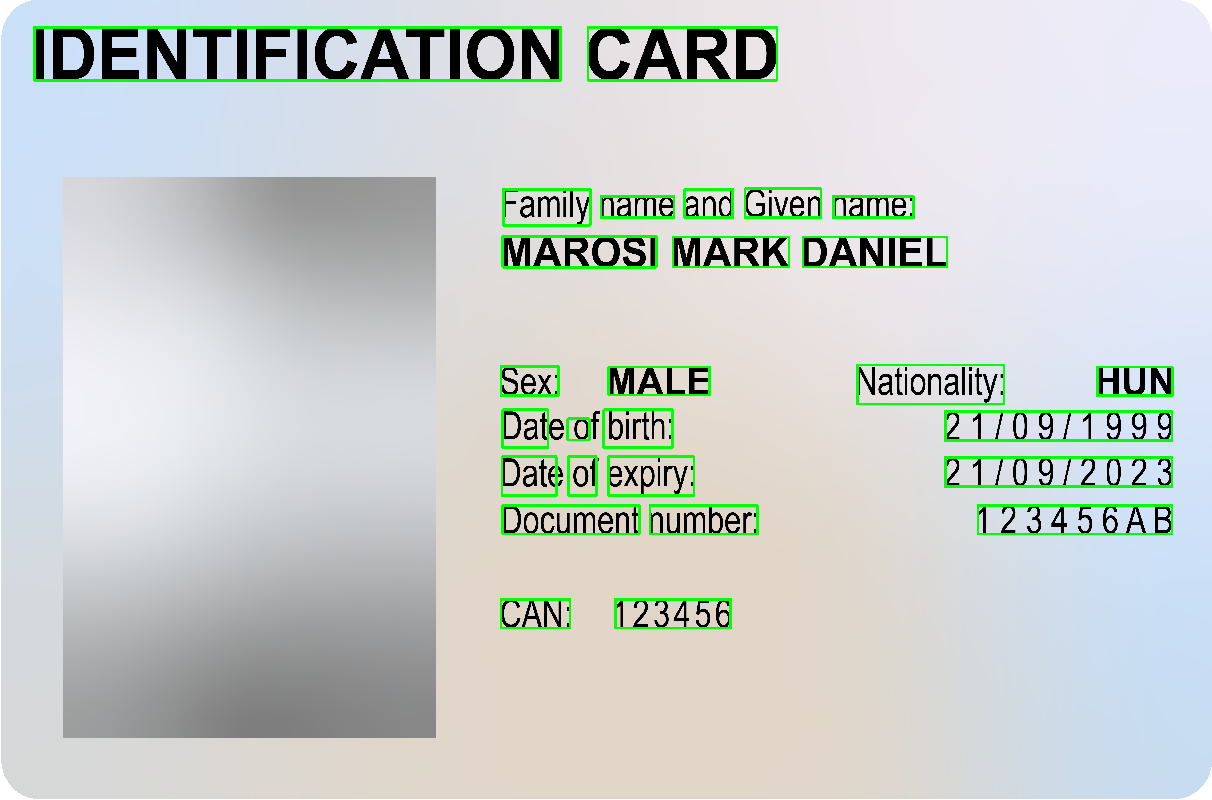
\includegraphics[scale=.4]{boxes_pytesseract.eps}}
    \caption{A függvényhívás eredménye, a Pytesseract által kinyert adatok}
\end{figure}

\begin{verbatim}
def generate_img_with_bounding_boxes_on_words(ocr_result):
    img = cv2.imread(ID_CARD_PATH)

    for i in range(len(ocr_result['text'])):
        if float(ocr_result['conf'][i]) >= CONF_LEVEL:
            (x, y, w, h) = (ocr_result['left'][i],
                            ocr_result['top'][i],
                            ocr_result['width'][i],
                            ocr_result['height'][i])
            img = cv2.rectangle(img, (x, y),
                (x + w, y + h), (0, 255, 0), 10)

    output_img_to_window(img)
\end{verbatim}

\begin{verbatim}
def output_img_to_window(img):
    cv2.namedWindow("output", cv2.WINDOW_NORMAL)
    cv2.imshow("output", img)
    cv2.waitKey(0)
    cv2.destroyAllWindows()
\end{verbatim}

\subsection{Az EasyOCR könyvtár bemutatása}

Az EasyOCR könyvtár is egy nyílt forráskódú \cite{easyocr}, ingyenesen használható OCR könyvtár. A Tesseracttól független, eltérő az implementációja, összességében nagyobb pontosságot képes biztosítani bizonyos esetekben, hátulütője az, hogy nagyobb inputokra lassabb, mint a Tesseract.

Az EasyOCR importálása után először példányosítani kell egy objektumot az \newline \emph{easyocr.Reader()} konstruktorhívással, majd rendelkezésünkre állnak az EasyOCR metódusai. Ezek közül a szakdolgozat szempontjából a \emph{readtext()} metódus a legfontosabb, ennek egyetlen paramétere az kép elérési útvonala, melyről szöveget szeretnénk kinyerni.
A metódus egy listával tér vissza, melyben minden listaelem egy szó vagy szövegrészlet, melyet az OCR a karakterek egymáshoz viszonyított pozíciója alapján összefüggőnek ítélt. Minden egyes listaelem további elemeket tartalmaz. Első helyen egy listát, ami az adott szöveget körülvevő téglalap négy sarkának koordináta-párjait tárolja, második helyen magát a felismert szöveget, a harmadik pozíción a pedig tizedestört alakban kifejezve azt, hogy az OCR hány százalékban biztos abban, hogy a kinyert szöveg egyezik a képen látható szöveggel.

\begin{tcolorbox}
    \begin{center}
        \begin{tabular}{ c c c }
         bounding box coordinates & text & confidence \\ 
         {[}{[}329, 78{]}, {[}3551, 78{]}, {[}3551, 350{]}, {[}329, 350{]}{]} & Nationality: & 0.97 \\
        \end{tabular}
    \end{center}
\end{tcolorbox}

\noindent
Ahogyan azt a pytesseract könyvtár eredményén megtettem, itt is szemléltetésképpen írtam egy metódust, ami a bemenetként adott képen megjeleníti a felismert szavakat, összefüggőnek vélt karakterláncokat.

\pagebreak

\begin{figure}[h]
    \centerline{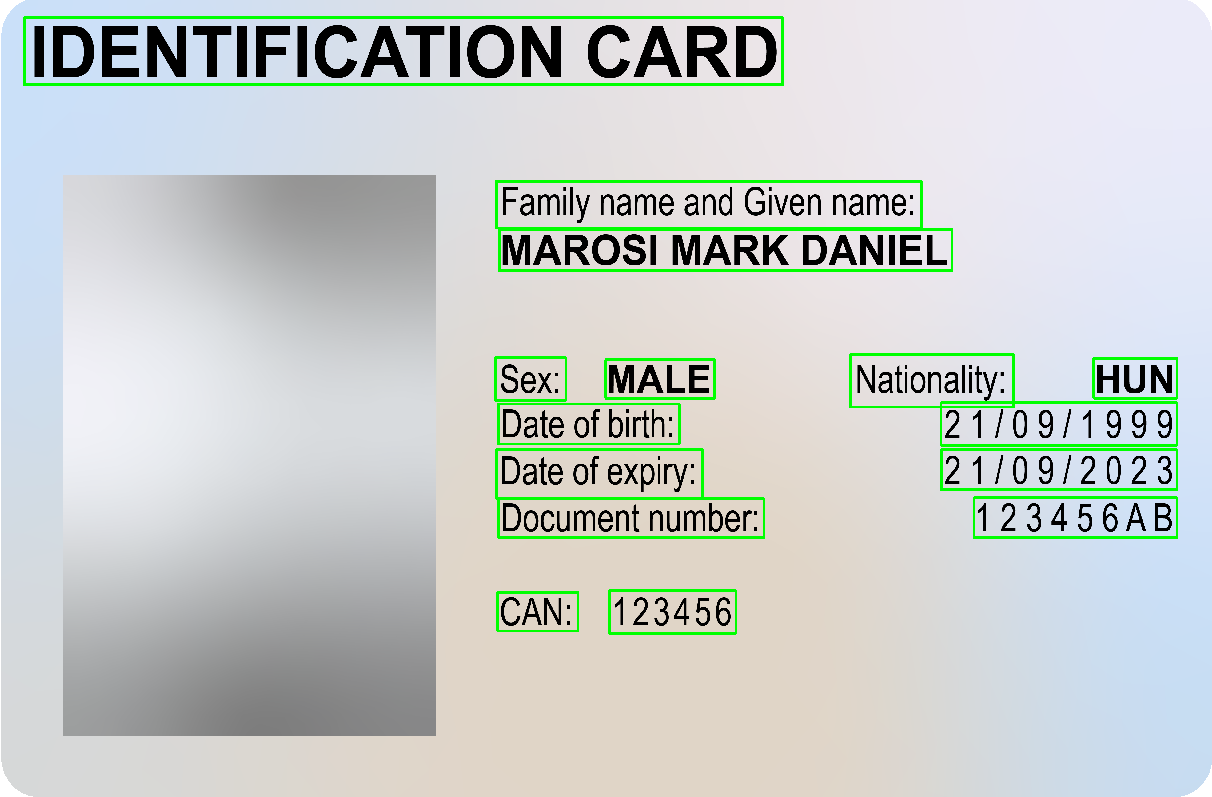
\includegraphics[scale=.4]{boxes_easyocr.eps}}
    \caption{A függvényhívás eredménye, az EasyOCR által kinyert adatok}
\end{figure}

\begin{verbatim}
def generate_img_with_bounding_boxes_on_words(ocr_result):
    img = cv2.imread(ID_CARD_PATH)

    for text_row in ocr_result:
        bottom_left = tuple(text_row[0][0])
        top_right = tuple(text_row[0][2])
        img = cv2.rectangle(img, bottom_left, top_right, 
                            (0, 255, 0), 10)

    cv2.namedWindow("output", cv2.WINDOW_NORMAL)
    cv2.imshow("output", img)
    cv2.waitKey(0)
    cv2.destroyAllWindows()
\end{verbatim}

\noindent
Ha összehasonlítjuk a két bemutatott könyvtár által adott eredményeket és összevetjük az utóbbi két képet, megfigyelhető, hogy valóban van eltérés a két metódus eredménye között. A legfőbb különbség a szövegrészletek szegmentáltságából adódik: míg az EasyOCR az egymáshoz közel álló szavakat, karakterláncokat sokkal inkább egy egységként dolgozza fel, addig a Pytesseract karakter alapon vizsgálja a dokumentumot, kevésbé érzékeny a kontextusra, ebből adódóan szavakra bontva dolgozza fel a képen olvasható szöveget.

\section{A dokumentum előfeldolgozása}

Ahogyan "Az OCR pontosságának javítása bemeneti oldalon" című fejezetben kifejtettem, a lehető legpontosabb OCR kimenet eléréséhez szükségünk van a bemeneti kép előfeldolgozására pár lépésben az OpenCV nevű ingyenes könyvtár különböző metódusainak használatával. \cite{opencv_functions}
Mivel a bemeneti dokumentum lehet színes, így először a színek eltüntetésével kezdtem, hiszen a színek a szövegkinyerés szempontjából felesleges információt hordoznak. Ezt az OpenCV \emph{cvtColor()} nevű metódusával értem el, melynek paraméterei egy kép, és az a színtér, melyre konvertálni szeretnénk. A mi esetünkben ez a színtér a \emph{COLOR\_RGB2GRAY}, ami az RGB színeket a szürke árnyalataivá konvertálja.

\begin{verbatim}
def convert_to_grayscale_image(image):
    return cv2.cvtColor(image, cv2.COLOR_RGB2GRAY)
\end{verbatim}

\noindent
Következő lépésként a zajeltávolítás volt a célom. Egy zajos kép nagy mértékben ronthatja a kimenet pontosságát, mivel az OCR a zajos, szemcsés részeket is az adott karakter részének határozhatja meg. A zajeltávolítás legegyszerűbb módja a kép kis mértékben történő elmosása, mivel így a zajos részeket összemossuk és jobban beleolvad a háttérbe, cserébe, ha tényleg csak kevés elmosást alkalmaztunk, a karakterek szélei csak kis mértékben veszítenek az élességükből, ezzel továbbra is fenntartva a felismerhetőséget.
Erre a célra a \emph{medianBlur()} metódust hívtam meg az OpenCV könyvtárból, melynek paraméterei a kép és egy 1-nél nagyobb páratlan szám, mely az elmosáshoz használt digitális rekesz lineáris méretét adja meg.

\begin{verbatim}
def remove_noise(image):
    return cv2.medianBlur(image, 5)
\end{verbatim}

\noindent
Utolsó lépésben a képen található szöveget elkülönítjük a háttértől, amennyire csak lehet. Ezt az OpenCV \emph{threshold()} nevű metódusával érhetjük el, melyet általában arra használnak, hogy egy szürkeárnyalatos képet két színből álló képpé konvertáljanak. A függvény paraméterei a kép, egy küszöbérték (\emph{threshold}), egy maximum érték (\emph{maxval}), és a küszöbérték típusa.
Különböző célokra különböző küszöbérték típusok léteznek \cite{opencv_threshold}, számomra a \emph{THRESH\_BINARY} a legmegfelelőbb.
A \emph{THRESH\_BINARY} küszöbérték típus számítási elve:
\begin{equation}
output(x,y)=
    \begin{cases}
        maxval, & \text{ha}\ input(x,y)>threshold \\
        0, & \text{egyébként}
    \end{cases}
\end{equation}

\noindent
A képletből kiolvasható, hogy amennyiben a vizsgált pixel színe a küszöbértéknél nagyobb, akkor a szín átírásra kerül, és a maxvalue értékét fogja felvenni, egyéb esetben az új értéke 0 lesz.
Ahhoz, hogy a szöveg jól elkülönüljön a háttértől, a lehető legszűkebb küszöbértéket kell megadnunk, így a \emph{threshold} paraméter a mi esetünkben 0 lesz. A \emph{maxvalue} az a szín, amit a küszöbértéknél nagyobb, azaz kiszűrni kívánt képpontok (ebben az esetben a dokumentum háttere) fog felvenni, ez a mi esetünkben 255 lesz, azaz fehér.

\begin{figure}[h]
    \centerline{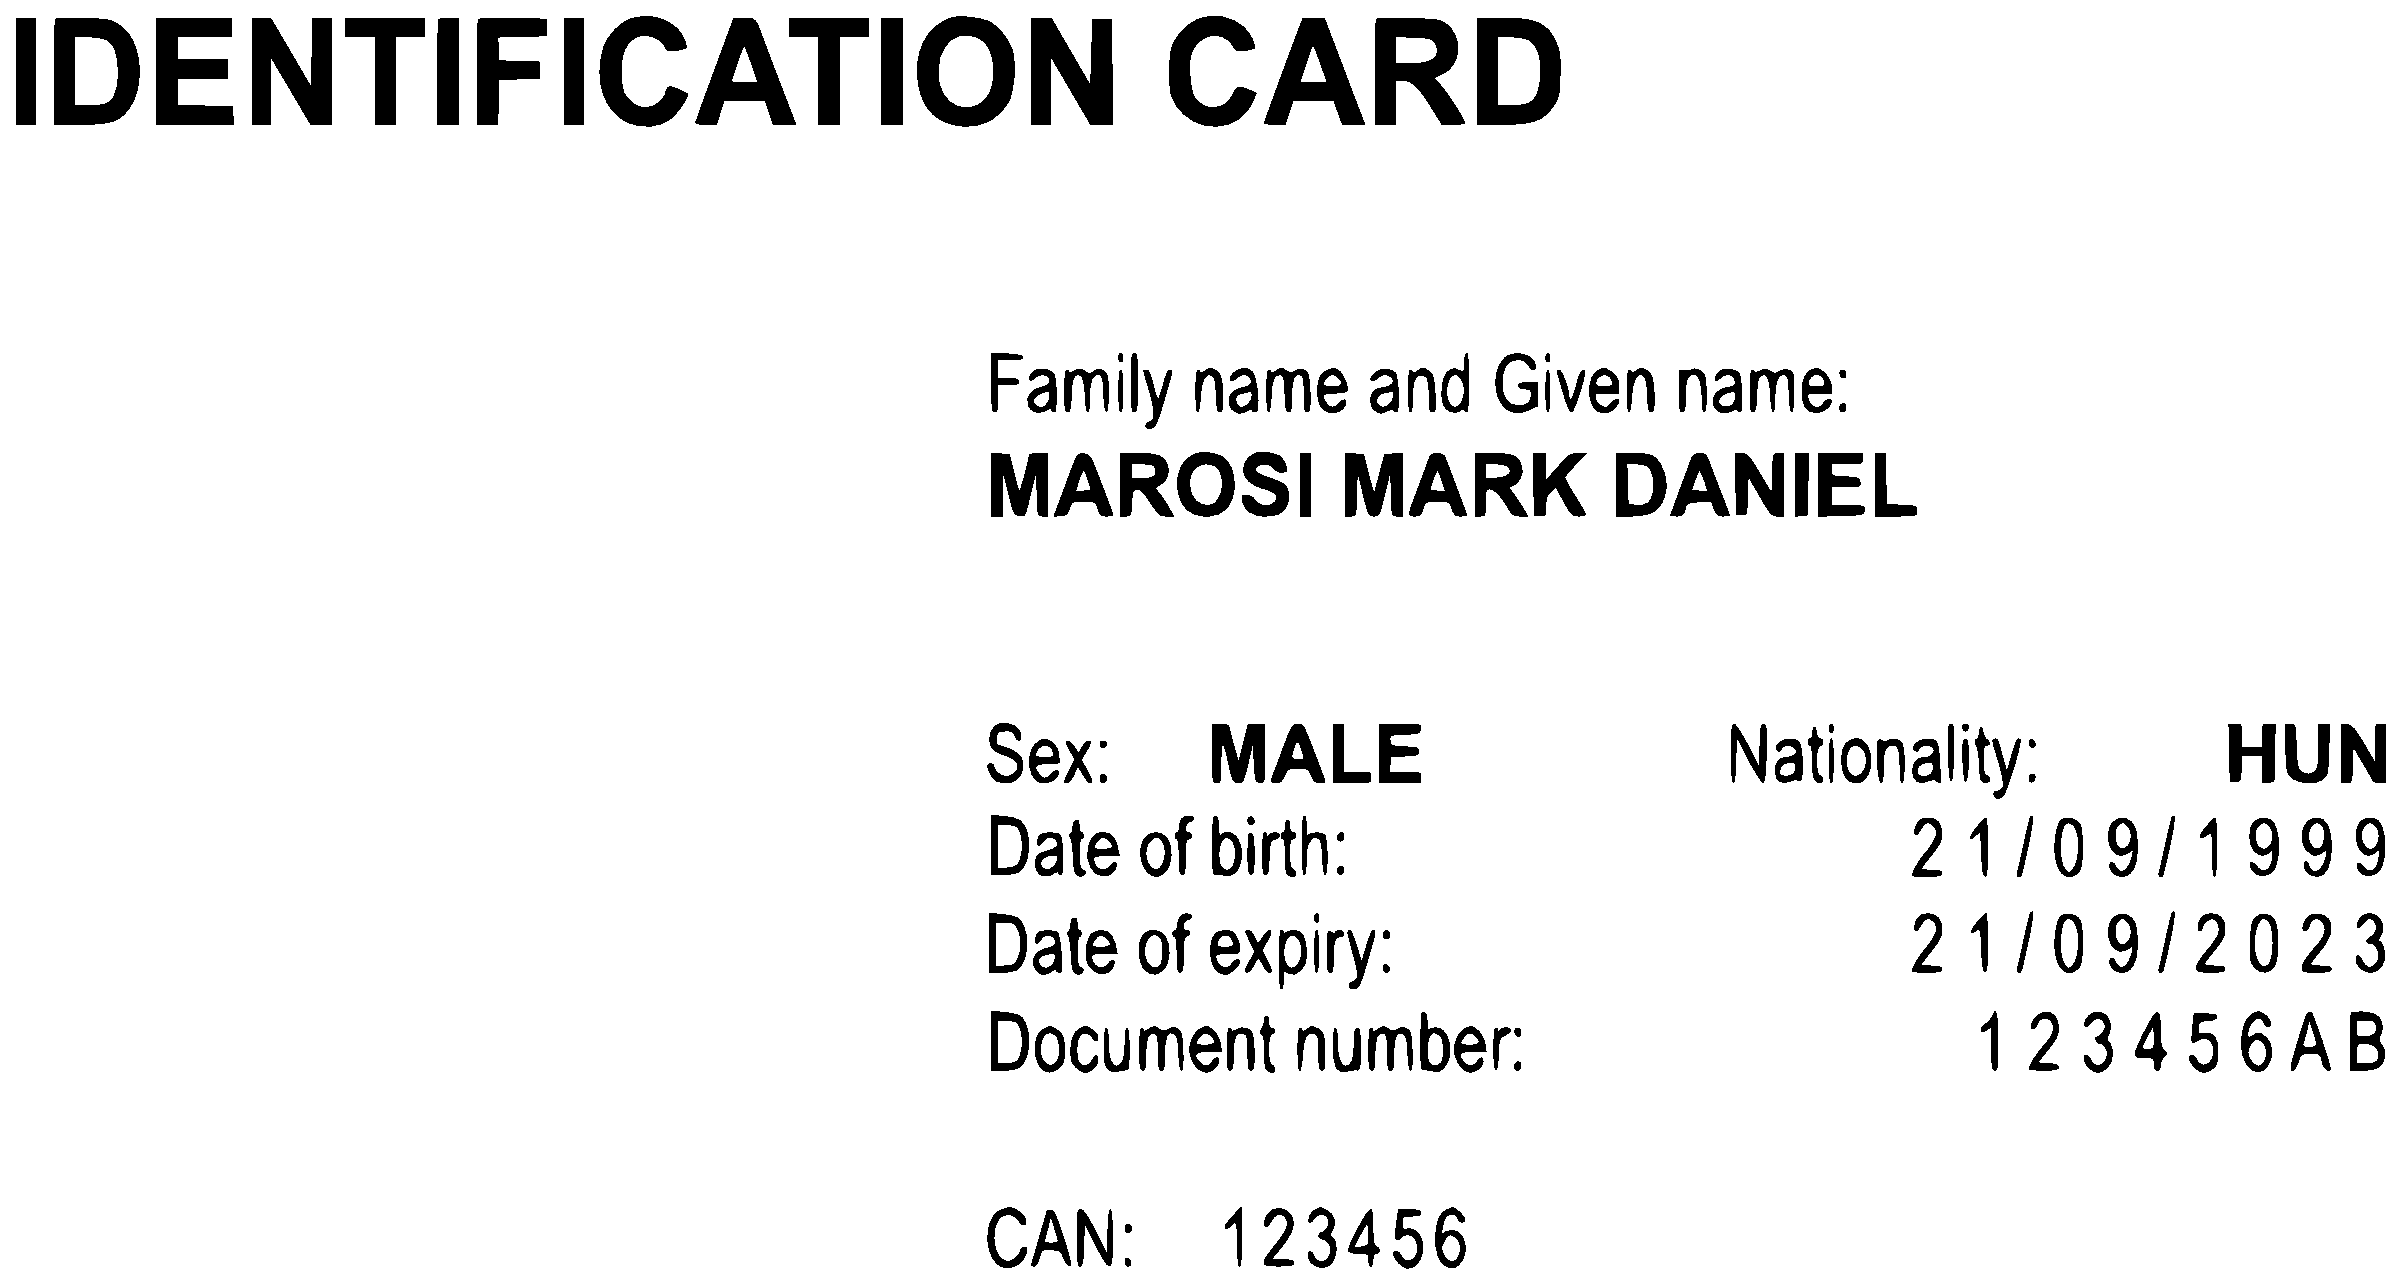
\includegraphics[scale=.25]{preprocessed_image.eps}}
    \caption{A három előfeldolgozó metódus futása utáni állapot}
\end{figure}

\noindent
A három képfeldolgozó metódus lefuttatása után elértem, hogy a szöveg jól elkülönüljön a háttértől, a karakterek könnyen felismerhetőekek legyenek, és ne maradjon a szövegfelismerés szempontjából irreleváns jelentést hordozó adat a dokumentumon.

\section{Adatstruktúra felállítása és feltöltése}

Ahhoz, hogy a képről kinyert szöveget hatékony módon, könnyen kereshető és osztályozható formában tudjam tárolni, az objektum orientált programozás egyik alappillérét, az osztályokat hívtam segítségül. Egy osztály többek között rendelkezhet tulajdonságokkal és definiálhat metódusokat. A dokumentumról kinyert adatoknak sok közös tulajdonságuk van. Mindegyik magával hordoz egy karakterláncot, valamint a dokumentumon való elhelyezkedést leíró koordinátákat. Pythonban az adattagok definiálására és az értékeik kezdetleges beállítására a konstruktor szolgál.

\begin{verbatim}
class CardTextItem:
    def __init__(self, top_left, top_right, btm_left,
                 btm_right, text, conf):
        self.top_left = top_left
        self.top_right = top_right
        self.btm_left = btm_left
        self.btm_right = btm_right
        self.text = text
\end{verbatim}

A \emph{top\_left}, \emph{top\_right}, \emph{btm\_left} és \emph{btm\_right} adattagok rendre annak az alakzatnak a bal felső, jobb felső, bal alsó és jobb alsó pontjainak koordináta párjait jelölik, mely pontosan körbehatárolja az egybefüggően kinyert karakterláncot.

Azzal, hogy elkészült az adatstruktúra, már csak fel kell tölteni az OCR által kinyert adatokkal. Ehhez vissza kell emlékezni az EasyOCR könyvtár bemutatása című alfejezet során szemléltetett adatstruktúrára, melyben rendelkezésünkre áll a dokumentumról felismert összes karakterlánc. Ez egy olyan lista, melyben minden elem egy további struktúrát tartalmaz, benne a koordinátákkal, a szöveggel és a szöveg pontosságát becslő számmal. Ezt a listát szeretném úgy szétbontani, hogy minden elemét leképezem egy olyan objektummá, ami az előbb felállított adatstruktúra egy példánya, azaz minden egyes karakterlánc egy önálló objektum lenne.

\begin{verbatim}
def get_text_items_from_ocr_data(ocr_data):
    card_text_items = list()

    for i in range(len(ocr_data)):
        item_bl = ocr_data[i][0][0]
        item_br = ocr_data[i][0][1]
        item_tr = ocr_data[i][0][2]
        item_tl = ocr_data[i][0][3]
        item_text = ocr_data[i][1]

        text_item = cti.CardTextItem(item_tl, item_tr, 
                            item_bl, item_br, item_text)
        card_text_items.append(text_item)
\end{verbatim}

A metódusban végig iterálunk az OCR által kinyert adatokon, és az aktuális elemet tovább bontva a megfelelő adattaghoz rendeljük. Ezután létrehozunk belőle egy példányt, majd hozzáadjuk a kész, feltöltött objektumokat tároló listához. A metódus futása után a lista minden eleme egy OCR által kinyert karakterláncot tartalmazó objektum. Példaképpen, az általam készített minta személyi igazolványról kinyert adatok listájának első eleme a metódus futása után:

\begin{tcolorbox}
    Text: IDENTIFICATION CARD

    top\_left: [333, 350], top\_right: [3551, 350]

    btm\_left: [333, 78], btm\_right: [3551, 78]
\end{tcolorbox}

\section{Kulcs-érték párok azonosítása}

A program írása során ezen a ponton már nem volt triviális az, hogy milyen irányban folytatssam a fejlesztést. A dokumentumról az EasyOCR segítségével sikerült kinyerni minden szöveget, és bár sikerült ezeknek egy adatstruktúrát felállítani, de ezt leszámítva, a végeredményt tekintve ezen a ponton még csak azt sikerült elérni, amire az interneten található, ingyenes applikációk is képesek. A következő, és egyben a szakdolgozat szempontjából legfontosabb lépés az adatok osztályozása, az összetartozó adatpárok megkeresése.

A dokumentumra tekintve megállapíthatjuk, hogy a legtöbb adat igazából egy adatpár, ahol az egyik nevezhető kulcsnak, a másik pedig értéknek. Például a \emph{Document Number} szöveg az egy kulcs, mivel egyértelműen azonosítható belőle, hogy milyen jelentést hordoz. Az \emph{123456AB} karakterlánc pedig ennek a kulcsnak az értéke. Azért érték, mert önmagában nem hordoz jelentést, de ha hozzákapcsoljuk a kulcsához, onnantól tudjuk, hogy mit jelent. Tehát a kulcs az felfogható egy egyedi azonosítóként, aminek az értéke az azonosított adat. Viszont a kulcs-érték párokba történő rendezés nem egy triviális feladat, és több módszer is felmerült a probléma megoldására.

Az egyik irány az a reguláris kifejezésekre épült volna, a felismert szövegeket bizonyos tulajdonságok alapján próbálta volna a program besorolni egy előre definiált kulcs halmazhoz. Például igazolványszámot a szabvány alapján (adott mennyiségű betűk és számok, meghatározott sorrendben), vagy dátumokat a benne szereplő számok és elválasztó jelek alapján. De ehhez előre definiálni kellett volna, hogy milyen kulcsok szerepelhetnek a dokumentumon, ami eléggé megkötötte volna a felhasználási lehetőségeket, továbbá a reguláris kifejezésekben kevés kihívást, kisebb rugalmasságot és pontosságot véltem felfedezni. Ennek ellenére a reguláris kifejezések használatának ötletét nem felejtettem el, és a későbbiekben még felhasznátam.

Mindenképpen szerettem volna felhasználni az OCR által kinyert szövegekhez tartozó koordinátákat, így a következő ötletem az volt, hogy egy előre meghatározott sablon segítségével felismerhetőek legyenek az összetartozó adatok. A sablon úgy működött volna, mint egy generikus verzió a vizsgált dokumentumból, amin előre meg lett volna adva, hogy milyen koordináták között milyen adatot kell keresni. Feltételezve, hogy a vizsgált dokumentum illeszkedik a sablonra, könnyen meghatározható lett volna, hogy melyik karakterlánc milyen jelentést hordoz. Viszont ez is egyfajta kötöttséget vont volna maga után, hiszen ha kicsit változik a dokumentum felépítése, akkor a sablonon is módosítani kellene, hogy a kinyert adatok jelentése továbbra is meghatározhatóak maradjanak. Emiatt ezt a lehetőséget is kizártam.

Végül egy saját magam által írt algoritmus mellett döntöttem, ahol nincsenek előre meghatározva a kulcsok, és az értékek elhelyezkedése sincsen megkötve, mint egy sablonnál. Ebből kifolyólag az algoritmusnak képesnek kell lennie megállapítania minden adatról, hogy az kulcs, vagy érték. Ez természetesen nem egy egyszerűen megállapítható és eldönthető kérdés, meg kellett határoznom, hogy milyen feltételek mellett számít valami kulcsnak vagy értéknek. Sok dokumentum típust végignézve megfigyeltem, hogy a kulcsok általában vagy az értéktől balra, vagy az érték felett helyezkednek el. Ez természetesen nem fed le minden esetet, de egy elég jó kiindulási pont volt az algoritmus implementálásához. 

Az algoritmus végig iterál a teljes listán, mely a kinyert szövegeket tároló objektumokat tartalmazza. Minden iteráció első lépése az, hogy keressünk az objektumok közül egyet, amire nagy biztossággal rámondható, hogy az egy kulcs. Ennek a megállapítására írtam a find\_next\_key metódust, mely az összes objektumot összehasonlítva megkeresi azt, amelyik a koordinátái alapján a többihez képest legjobban balra és legjobban felül van, máshogy fogalmazva megkeresi a bal felső sarokhoz legközelebb eső elemet. Mivel feltételeztem, hogy a kulcsok minden esetben vagy az értkékek bal oldalán, vagy az értékek felett vannak, így elméleti szinten az algoritmus nem találhat értéket, hiszen annak kulcsa mindenképpen közelebb lesz a bal felső sarokhoz.

Először a \emph{CardTextItem} objektumba fel kellett vennem 4 új adattagot: \emph{is\_examined}, \emph{assigned\_to}, \emph{is\_key}, \emph{is\_value}. Mind a négy adattag kezdetben 0-ra inicializálódik. Az is\_examined egy logikai változóként viselkedik, és azt jelzi, hogy a kulcs-érték pár keresés lefutott-e már rá. Erre azért volt szükség, hogy ha az adott szövegre futó keresés nem talált hozzá tartozó párt, akkor jelezve legyen, hogy ez nagy eséllyel egy olyan szöveg, mely csak tájékoztató jellegű, nem pedig egy fontos adat. Ilyen például a példa igazolványon az \emph{IDENTIFICATION CARD} szöveg, mely nem lesz kulcs, hiszen érték sem tartozik hozzá.
Az \emph{assigned\_to adattag} segítségével lesznek összekapcsolva azok az objektumok, amik a kulcs-érték pár keresés során egymáshoz lettek rendelve. Maga az adattag hozzá kapcsolt másik objektumra fog mutatni. Az \emph{is\_key} és az \emph{is\_value} adattagok pedig szintén logikai változókként funkcionálnak, jelezvén, hogy az adott objektum kulcsként vagy értékként lett felismerve.

\newpage

\begin{verbatim}
def find_next_key(items):
    next_key = next(item 
                    for item 
                    in items 
                    if item.is_examined == 0)

    for item in items:
        if item.is_examined == 0:
            if item.top_left[1] < next_key.top_left[1]:
                next_key = item
\end{verbatim}

A metódus paraméterben megkapja az objektumok listáját, és a \emph{next()} beépített függvény és egy szűrés segítségével kiválasztja a listából az első olyan objektumot, amit még nem vizsgáltunk. Ezután végig iterálva az objektumokon összehasonlítást végez a bal felső sarok Y koordinátája alapján. Az iteráció végére megkapjuk a dokumentum tetejéhez legközelebb eső (az Y tengelyen legmagasabban lévő) objektumot.
Ezen a ponton felmerült egy fontos kérdés. Amennyiben a legfelül elhelyezkedő objektummal egyező magasságban található még több is, akkor a leginkább balra esőt fogjuk kulcsként címkézni. De olyan szélsőséges eset is előfordulhat, hogy nem pont azonos Y koordinátán, de nagyon pici eltéréssel szintén található egy másik objektum, tőle balrább elhelyezkedve, akkor őt kell kulcsként címkézni.
Mivel nem feltételezhetjük, hogy a dokumentumon egymás mellett elhelyezkedő szövegek 1 pixel pontosságra egy vonalban vannak, továbbá azt sem, hogy az egymás alatt lévő szövegek bal széle pontosan egy függőlegesen húzott vonalra illeszkednek, így be kellett vezetnem egy olyan tűréshatár értéket, melyet hozzáadva illetve kivonva az éppen vizsgált X vagy Y értékből megkapjuk a tűréshatár intervallumot.
Amennyiben ezen az intervallumon belül találunk újabb kulcsokat, azokról meg kell állapítani, hogy közelebb vannak-e a dokumentum bal széléhez, mint amit eddig találtunk. A find\_next\_key metódus az alábbi sorokkal egészül ki:

\begin{verbatim}
upper_bound = next_key.top_left[1] + THRESHOLD
lower_bound = next_key.top_left[1] - THRESHOLD

for item in items:
    if item.is_examined == 0:
        if lower_bound <= item.top_left[1] <= upper_bound:
            if item.top_left[0] < next_key.top_left[0]:
                next_key = item
\end{verbatim}

\newpage

A \emph{THRESHOLD} konstans változó értékének meghatározása próbálgatással történt. A 40-es érték bizonyult minden esetben jónak, ez még az a tűréshatár, amibe az egymás mellett és alatt elhelyezkedő objektumok beleesnek, de azok már nem, amik a keresés eredménye szempontjából helytelenek lennének. Ezt a konstanst többször is használni fogom a kulcs-érték párok felderítése során.

A \emph{find\_next\_key()} metódus visszatérési értéke az az objektum lesz, ami Y tengelyen a legmagasabban helyezkedik el. Amennyiben ezen objektum X koordinátájának a tűréshatár intervallumán belül találunk egy vagy több másik, tőle  balra eső objektumot, úgy azzal térünk vissza, amelyik ezek közül a legközelebb van a dokumentum bal széléhez. Tehát a metódus visszatér egy objektummal, melyről innentől feltételezzük, hogy kulcs. 
Azért nem jelenthető ki, hogy kulcs, mert csakis onnantól címkézünk egy objektumot kulcsként, ha megbizonyosodtunk róla, hogy tartozik hozzá érték. Ezen a ponton ebben még nem lehetünk biztosak.

A folyamat következő lépése a \emph{find\_value\_for\_key()} nevű metódus, melynek paraméterei az előbb talált objektum, mely feltételezhetőleg kulcs, valamint a teljes objektumok listája. A futás rögtön azzal kezdődik, hogy az objektum \emph{is\_examined} adattagját 0-ról 1-re állítja, ezzel jelölve, hogy a párkeresési algoritmus már meg volt hívva a kulcsra. Ennek célja, hogyha nem találunk hozzá tartozó értéket, akkor se vizsgáljuk többet. A metódus ezután 2 fő lépcsőből áll. Az első, hogy elindít egy jobbra történő keresést, melynek ha van eredménye, akkor az a kulcstól jobbra talált legközelebbi objektum.
Innentől tudjuk, hogy az eddig kulcsnak vélt objektum valóban kulcs, hiszen találtunk egy objektumot mellette, mely feltételezhetően a hozzá tartozó érték. Amennyiben a jobbra keresésnek nem lett eredménye, úgy egy lefelé történő keresés indul. Amennyiben a kulcsnak vélt objektum alatt sem találtunk másik objektumot, akkor a metódus futása véget ér anélkül, hogy a kulcsnak vélt objektumot valóban kulcsként címkéztük volna, és értéket rendeltünk volna hozzá. Ebből megállapítható, hogy az objektumhoz valószínűleg nem tartozik érték.
Ilyen például az \emph{IDENTIFICATION CARD} szöveg, se tőle jobbra, se alatta nem helyezkedik el hozzá kapcsolható érték.
Mivel a kulcs keresés mindig a bal felső objektumokból indul ki, így teljesen felesleges lenne balra illetve felfelé történő keresés, hiszen ott már nem találhatunk semmit. Ez természetesen hátrány egy olyan dokumentumnál, melyről nem mondható el, hogy a kulcsok minden esetben az értékek bal oldalán, vagy felettük találhatóak.

A \emph{search\_right()} metódus ugyanazokkal a paraméterekkel rendelkezik, mint a \break \emph{find\_value\_for\_key()}. Futása során először kiszámolja a tűréshatár intervallumot, majd ezen belül keres egyéb olyan objektumokat, melyek nem voltak még vizsgálva, és nincsenek más objektumhoz rendelve. Továbbá feltétel az is, hogy a kulcshoz képest nagyobb X koordinátával rendelkezzen, azaz tőle jobbra helyezkedjen el a dokumentumon.
A talált objektumokat egy listában gyűjtjük, és a jobbra keresés végén, amennyiben a listában nincs elem, akkor tudjuk, hogy nem volt objektum a kulcstól jobbra. Ebben az esetben egy lefelé történő keresés indul. Amennyiben csak egy objektum van a találatok listájában, úgy visszatérünk azzal az objektummal. Ha a találatok listája több elemet is tartalmaz, akkor a \emph{get\_closest\_item\_right()} függvény fog hívodni, mely a listát kapja paraméterül, és a koordináták alapján visszaadja azt, amelyik jobbról a legközelebb található a kulcshoz.

A \emph{search\_below()} metódus ugyan úgy működik, mint a search\_right, csak nem jobbra irányul a keresés, hanem a kulcstól lefelé. Ha a lefelé történő keresés során több objektumot is találunk, akkor hasonlóan, mint a search\_right metódusban, megkeressük azt, ami a legközelebb van a kulcshoz, csak nem az X tengelyről, hanem az Y-ról, a \emph{get\_closest\_item\_below()} metódus segítségével.

A kulcs-érték keresési folyamat belépési pontja a \emph{find\_key\_value\_pairs()} metódus. Ebben egy while ciklus és egy listaszűrés felel azért, hogy egy objektumon legfeljebb egyszer menjen végig a párkereső algoritmus.

\begin{verbatim}
def find_key_value_pairs(items):
    while any(item.is_examined == 0 for item in items):
        next_key = find_next_key(items)
        find_value_for_key(next_key, items)
\end{verbatim}

\noindent
Az \emph{any()} beépített listaszűrő metódus igazzal tér vissza, ha a lista legalább egy olyan objektumot tartalmaz még, ami nem volt vizsgálva. Ennek a helyességét a korábban tárgyalt \emph{find\_value\_for\_key()} metódus biztosítja. Tehát addíg, amíg van olyan objektum, melyet nem vizsgáltunk, keresünk egy kulcsot a dokumentumon a  \emph{find\_next\_key()} metódussal, majd a kulcshoz megkeressük a hozzá tartozó értéket a \emph{find\_value\_for\_key()} függvénnyel. Mivel Pythonban alapértelmezetten referencia szerinti paraméterátadás történik, így nem tér vissza semmivel ez a metódus, mert minden módosítást az eredeti objektumokon végzünk.
Ha már nincs több vizsgálatlan objektum, akkor visszatérünk a main függvénybe. Ezen a ponton a feladat már el volt végezve, hiszen minden objektumot megvizsgáltunk, megtaláltuk a kulcs-érték párokat. Viszont az eddig használt adatstruktúra innentől értelmét veszti, a \emph{CardTextItem} osztályból egyedül a \emph{text} adattag releváns számunka. Az egyszerűbb kezelés érdekében egy kulcs-érték párokat tároló adatstruktúra mellett döntöttem.

\newpage

\begin{verbatim}
def items_to_dict(card_text_items):
    result_dict = dict()

    for cti in card_text_items:
        if cti.is_key:
            result_dict[cti] = cti.assigned_to
        elif not cti.is_key and not cti.is_value:
            result_dict[cti.text] = "N/A"

    return result_dict
\end{verbatim}

Az \emph{items\_to\_dict()} metódus átrendezi az osztálypéldányokat egy dictionary adatstruktúrába, melynek minden kulcsa egy általunk kulcsnak vélt objektum \emph{text} adattagja (a dokumentumról kinyert karakterlánc), értéke pedig a kulcshoz tartozó érték text adattagja. Abban az esetben, ha egy adott példány se nem kulcs, se nem érték, azaz egy olyan elem, melyhez nem találtunk párt, akkor az átmásolás során őt felvesszük a dictionary egy kulcsaként, és az "N/A" szöveg kerül hozzá értékként, ezzel jelezve, hogy a szöveghez nem találtunk hozzá köthető másik objektumot. A példa igazolványon ilyen az \emph{IDENTIFICATION CARD} szöveg.
Ezekről meggyőződhetünk, ha végigiterálunk rajta és kiíratjuk minden elemét:

\begin{tcolorbox}
    Key: IDENTIFICATION CARD, Value: N/A

    Key: Family name and Given name:, Value: MAROSI MARK DANIEL

    Key: Sex:, Value: MALE

    Key: Nationality:, Value: HUN

    Key: Date of birth:, Value: 2 1/0 9 /1 9 9 9

    Key: Date of expiry:, Value: 2 1/0 9 /2 0 2 3

    Key: Document number:, Value: 1234 5 6 A B

    Key: CAN:, Value: 123456
\end{tcolorbox}

A minta igazolványról az adatok hibátlanul kerültek kinyerésre és a kulcs-érték párok megtalálása és párosítása is kiválóan sikerült. Viszont megfigyelhetjük, hogy bizonyos esetekben a szövegek formázásra, utólagos korrigálásra szorulnak.

\section{Adatok utófeldolgozása és exportálása}

Ha végignézzük a kulcs-érték párok kinyerésének eredményét, láthatjuk, hogy a kulcsok végén kettőspont szerepel. Ennek csak a dokumentumon volt szerepe, ez segített az emberi szemnek a kulcsokat összekötni az értékekkel. Viszont digitalizálva már szükségtelenek, így eltávolírásra kerülhetnek a Python függvénykönyvtárába beépített \emph{replace()} metódus segítségével.

A kulcsokhoz kapcsolt értékeket végigfutva néhány esetben azt vehetjük észre, hogy felesleges szóközök szerepelnek a karakterek között. Ezek még az OCR folyamat során kerültek ilyen formában kinyerésre. Ebből látszódik, hogy az egy gyenge pontja az EasyOCR könyvtárnak, ha egy karakterláncban az általánosnál nagyobb a betűköz. Utólagos javításra a legegyszerűbb módszer szintén a \emph{replace()} metódus lenne, de fontos észrevenni, hogy nem minden érték esetében tehetjük ezt meg. A név esetében például elrontanánk az adat helyességét azzal, hogy a vezetéknév és a keresztnév vagy keresztnevek közül eltűntetnénk a szóközöket. 
Ezért valahogyan ki kell szűrni azokat az adatokat, melyekről eltávolíthatóak a felesleges szóközök anélkül, hogy az a helyességük rovására menne.

Erre a célra mintaillesztést használtam. A mintaillesztés reguláris kifejezések segítségével történik, melyben megszabjuk, hogy milyen szabályokat és mintákat kell követnie az általunk vizsgált szövegnek. A mintaillesztés kimenete lehet elfogadó, amennyiben a szöveg teljes egészébena mintára illeszkedik, és megfelel a követelményeinknek, egyébként elutasító.
Tudjuk, hogy az olyan adatok, mint a nemzetiség kódja, a nem, a dátumok és a dokumentumszámok mind olyanok, melyek általános esetekben nem tartalmazhatnak szóközt. Így ezekre az adat kategóriákra írtam egy-egy reguláris kifejezést.

A dátumformátum a legbonyolultabb, hiszen a nap, hónap és év sorrendje változó, továbbá az elválasztó jelek is lehetnek eltérőek. Ehhez az interneten kerestem már kész reguláris kifejezéseket, \cite{date_regex} és azt kicsit átalakítva a programomba három konstans változóba felvettem. \emph{év}, \emph{hónap}, \emph{nap}, a másik a \emph{nap}, \emph{hónap}, \emph{év}, a harmadik pedig a \emph{hónap}, \emph{nap}, \emph{év} sorrendű megfelelőjét tárolja a reguláris kifejezésnek. Mind a három esetben az évet 4 számjegy, a hónapot és a napot pedig 2-2 számjegy jelöli. Egyéb eseteket nem vettem figyelembe, mivel ez a három nagyon nagy százalékban lefedi a különböző igazolványokon található formátumokat.

Az nemzetiséget jelölő ország kódjára saját reguláris kifejezést írtam. Az országok kódjai az ISO-3166 szabvány alapján 2 vagy 3 betűből állhatnak. \cite{country_codes} Az erre írt reguláris kifejezés így néz ki: \emph{\textasciicircum[a-zA-Z]\{2,3\}\$}. Ez egy egyszerű kifejezés, mely a kis- és nagybetűk között különbséget nem téve korlátozza, hogy a betűk számának 2 és 3 között kell lennie, semmilyen egyéb karakter nem megengedett a szövegen belül, de előtte és mögött sem.

A dokumentumszámoknál és egyéb azonsítóknál azt a feltételt szabtam meg, hogy a karakterláncnak tartalmaznia kell legalább 4 számot. Mivel ebbe beleesnek a dátumok is, így a szűrésnél figyelni kell, hogy először a dátum reguláris kifejezésére történjen a próbaillesztés, és ha arra nem illeszkedett a szöveg, akkor lehet próbálni a dokumentumszámra is. A dokumentumszám reguláris kifejezése: \emph{\textasciicircum(.*\textbackslash d)\{4,\}\textbackslash S*\$}. Bármilyen, bármennyi (akár nulla) karakter után kötelezően 4 vagy több szám kell, hogy szerepeljen, ami után bármennyi egyéb karakter állhat, akár egy sem.

Az utófeldolgozási folyamat lépéseit a \emph{post\_process\_text()} metódusban gyűjtöttem össze. A metódus végigmegy az összes szövegen, a kulcsokról leszedi a kettőspontot, az értékeket pedig megtisztítja a nem kívánatos szóközöktől, amennyiben a mintaillesztés eredménye alapján ez nem változtatja a szöveg helyességét.

\begin{verbatim}
def post_process_text(items_dict):
    new_items_dict = dict()

    for key, value in items_dict.items():
        cleaned = value.replace(' ', '')
        if matches_any_regex(cleaned):
            new_items_dict[key.replace(':', '')] = cleaned
        else:
            new_items_dict[key.replace(':', '')] = value

    return new_items_dict
\end{verbatim}

Az adatok exportálására a \emph{csv} nevű függvénykönyvár volt a segítségemre. A \emph{with open() as} segítségével erőforrást allokálok egy fájl írására, majd példányosítok egy writer objektumot, mely a beolvasott dokumentum mappájába fog létrehozni egy csv kiterjesztésű fájlt. A későbbi konfigurálhatóság érdelében a \emph{FILE\_EXT} konstans változóban tárolom a kiterjesztést leíró stringet. Az adatstruktúrán végigiterálva annak kulcsai és értékei beírásra kerülnek a fájlba pontosvesszővel elválasztva, sortöréssel lezárva. Ezzel lehetővé teszem, hogy excelbe is könnyen importálható legyen a kinyert adatok összessége, de bármilyen szerkesztővel megnyitva is könnyen olvasható legyen az emberi szemnek is a fájl tartalma.

\begin{verbatim}
def export_data_to_csv(path, data):
    filename = f"{path}/{name}_result.{FILE_EXT}"

    with open(filename, 'w') as file:
        writer = csv.writer(file, delimiter=';')

        for key, value in data.items():
            writer.writerow([key, value])
\end{verbatim}

\chapter{A kész alkalmazás bemutatása}

Mivel a program elkészítése során a fókusz a szövegfeldolgozáson és a kulcs-érték pár keresésen volt, így a felhasználói felület kapta a legkisebb figyelmet. Mivel ez egy olyan alkalmazás, melynek célzott, szűk körű közönsége van, és azok is inkább cégek vagy szervezetek, és nem magánszemélyek, így a lehető legegyszerűbb, minimalista felületet kapott a program.
Ennek megvalósítására a \emph{tkinter} nevű Python könyvtár eszközkészlete tűnt a legjobbnak, mely a \emph{Tcl/Tk} (Tool Command Language) \cite{tcl} eszközkészlet Pythonra írt interfésze. A \emph{tkinter} könyvtárnak is létezik néhány egyedi megvalósítása, ezek közül dizájn és színvilág szempontjából a \emph{customtkinter} \cite{customtkinter} tetszett a legjobban, így ezt a könyvtárat használtam a grafikus felhasználói felület elkészítésére.

\section{Az alkalmazás használata}
A felület az egyszerűség kedvéért mindössze egy gombot tartalmaz, mely kattintásra a fájlkezelőt nyitja meg, és várja, hogy a felhasználó tallózzon egy kép típusú fájlt. A fájl kiválasztása után a szövegkinyerési folyamat azonnal elindul, mely több másodpercet is igénybe vehet, erre a felhasználót egy "Process started, please wait..." üzenet figyelmezteti. Amint a szöveg kinyerése, feldolgozása és exportálása sikeresen megtörténik, a következő üzenet olvasható: "Process finished, CSV file saved to folder of the source image.".
Ha ezen a ponton bemenetként adott kép mappájába tekintünk, találnunk kell egy .csv kiterjesztésű fájlt, mely az alábbi módon van elnevezve: originalFileName\_result.csv (ahol originalFileName a bemenetként adott fájl neve). Ezzel biztosítottam azt, hogyha ugyan abból a mappából több fájlra is futtatásra kerülne a program, akkor minden fájlhoz megtalálható legyen a hozzá tartozó eredmény. Továbbá, ha egy fájlra többször futtatásra kerül a program, akkor ne sokszorozódjon a csv fájl, hanem íródjon felül az előző verzió.

A képen látható, hogy a felhasználónak lehetősége van bepipálni a "Show image with recognized text" jelölőnégyzetet. Amennyiben bejelölésre kerül a beállítás, a kulcs-érték párok megtalálása után felugró ablakban megjelenik az inputként adott kép, rajta zölddel bekeretezve minden felismert, egybefüggő karakterlánc, lilával pedig a kulcs-érték párok kerülnek összekötésre.
Így a felhasználónak lehetősége van vizuálisan is ellenőriznie, hogy melyik szóhoz mely érték tartozik, és melyek azok a szavak, melyekhez nem talált a program hozzá köthető párt.

\begin{figure}[h]
    \centerline{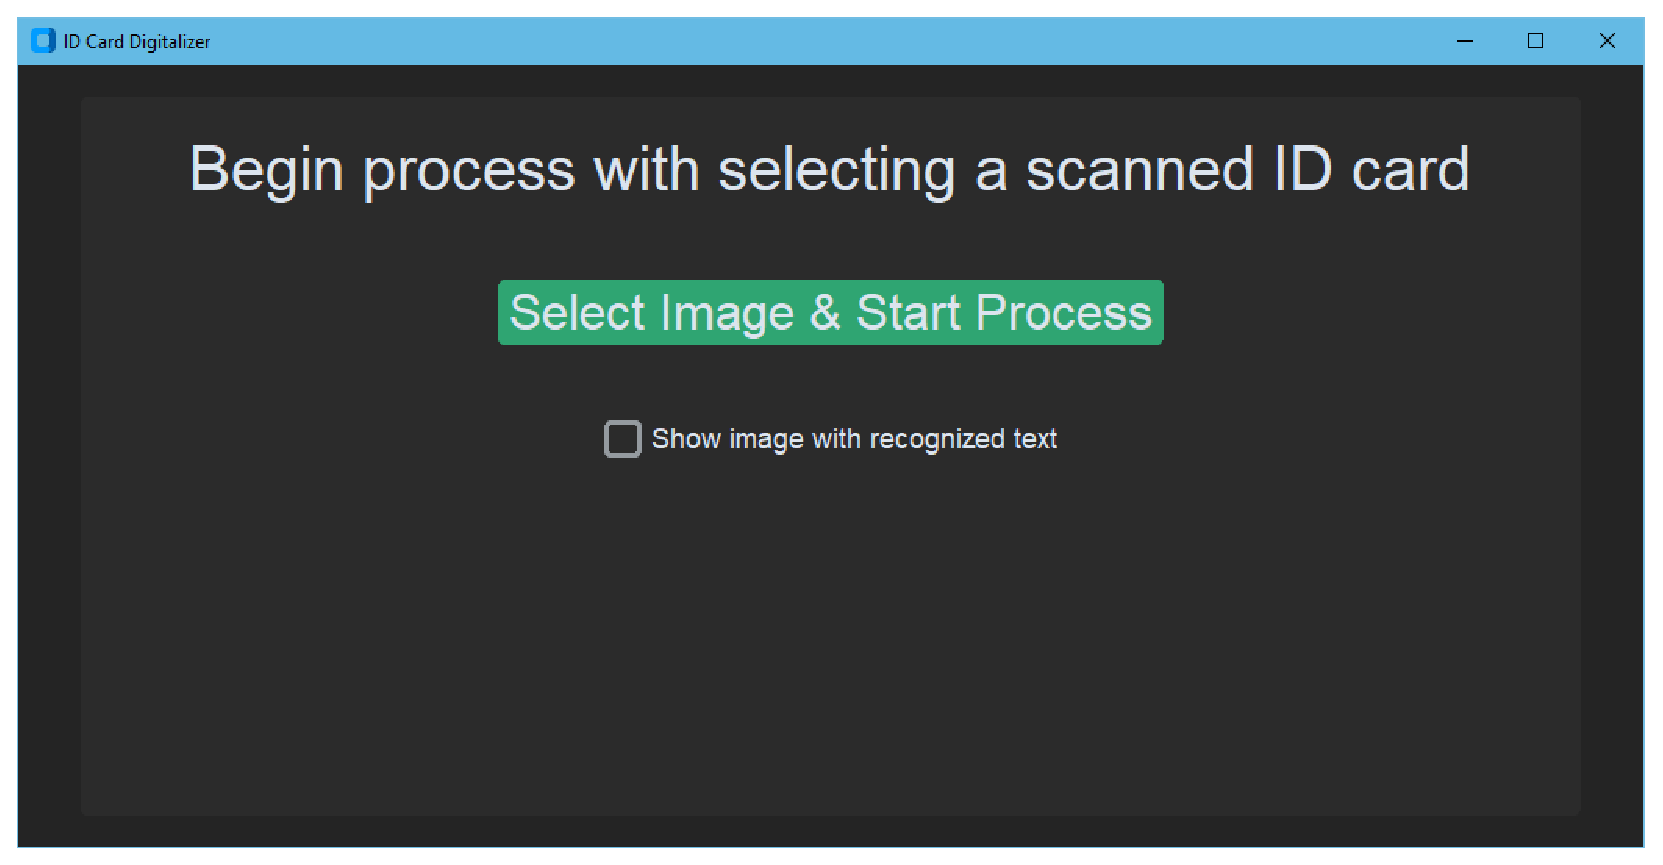
\includegraphics[scale=.5]{gui.eps}}
    \caption{A program grafikus felhasználói felülete}
\end{figure}

A program futása során keletkezhetnek hibák. Amennyiben az "Error while preparing and reading data." hibaüzenettel találja szembe magát a felhasználó, akkor vagy a kép előfeldolgozása, vagy az OCR folyamat során keletezett kivétel. Ha az "Error while processing data." üzenet jelenik meg, akkor az OCR eredményének leképezésénél, vagy a kulcs-érték párok keresésénél történt végzetes hiba.
A felhasználó találkozhat még az "Error while post-processing data." üzenettel, ami egyértelműen jelzi, hogy az utófeldolgozási lépés sikertelen volt egy nem várt hiba miatt. Amennyiben egy nem ennyire elkülöníthető folyamat során keletkezik hiba, akkor a "Something went wrong" üzenet jelenik meg. Ezek közül egyik hiba sem okozza a program leállását, így újra lehet próbálni a szövegkinyerési folyamatot.

\section{Eredmény bemutatása több bemenetre}

Az eddig használt példa igazolványról kinyert adatokat már bemutattam, de a program működésének validálásához több féle inputra is szükség van. Ezért készítettem két másik minta igazolványt, melyeken a szöveg eltérő módon van elrendezve.

\newpage

\begin{figure}[h]
    \centerline{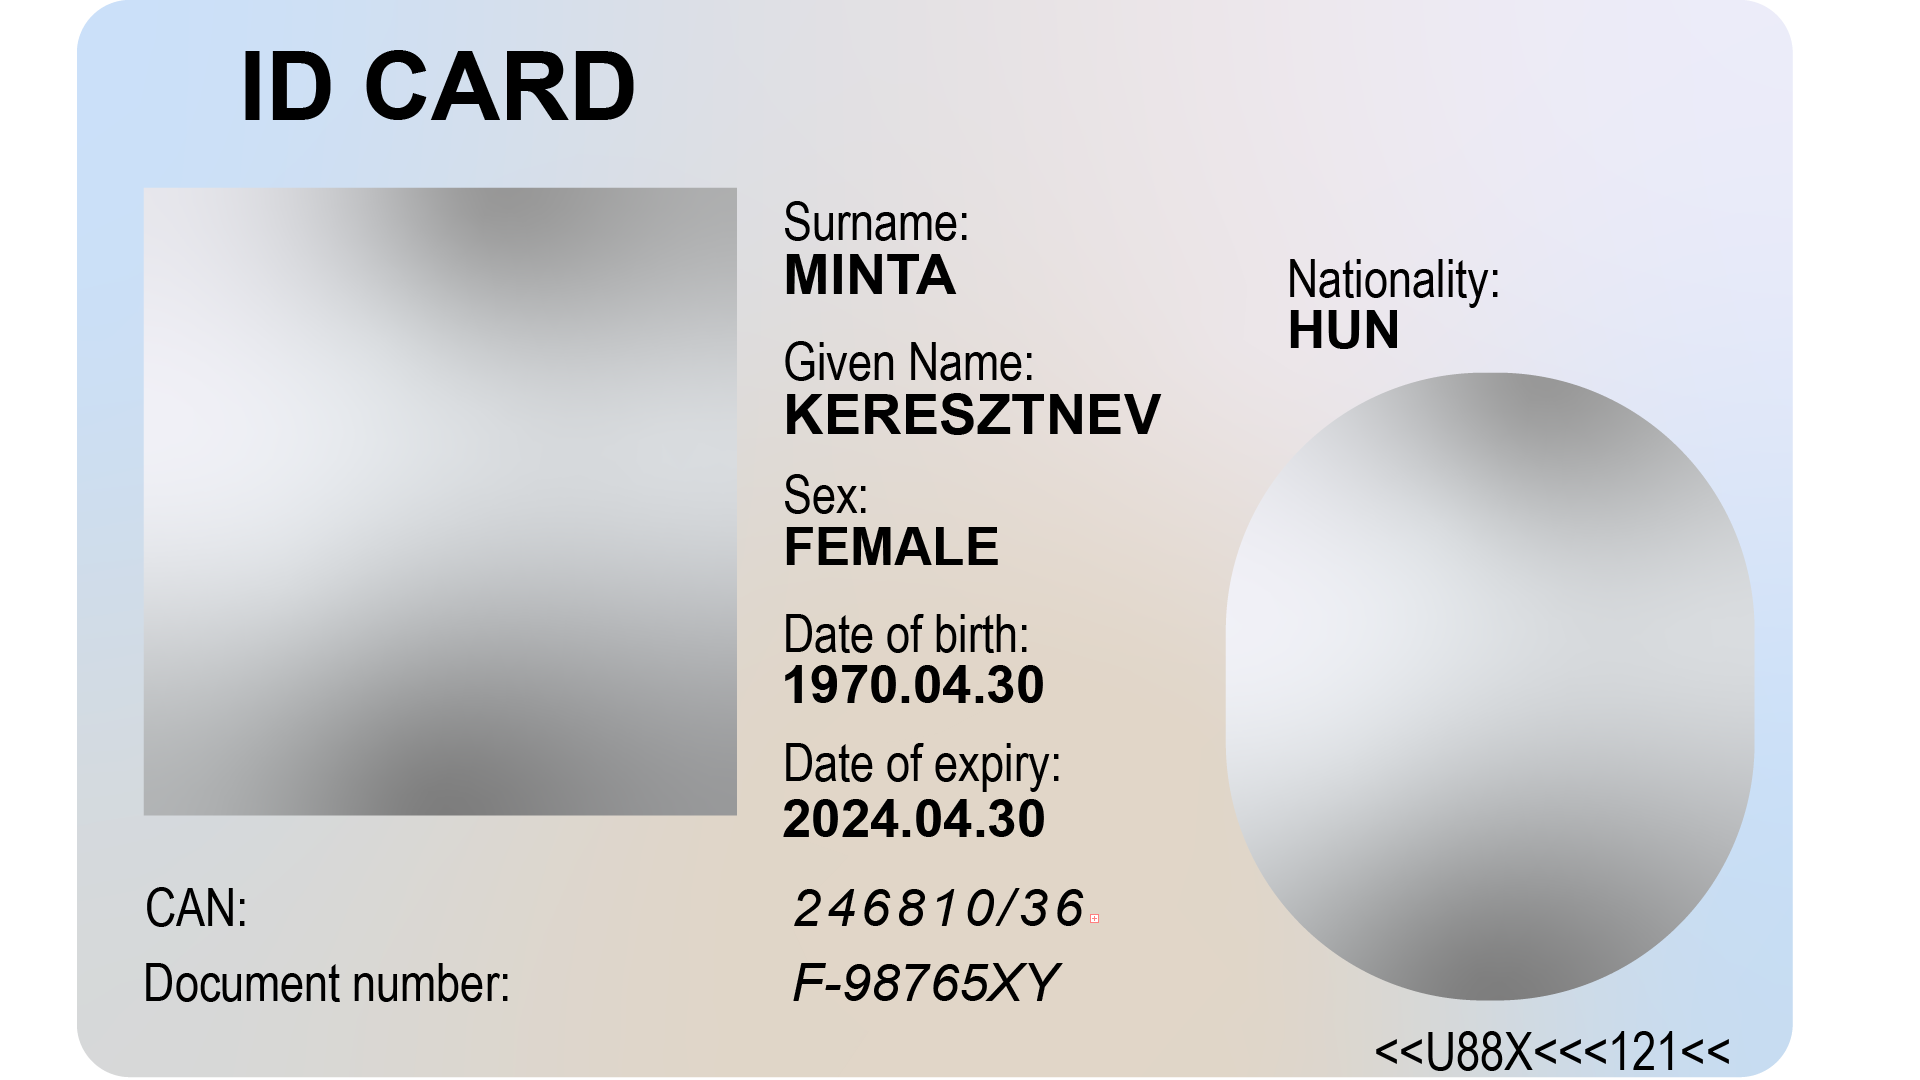
\includegraphics[scale=.2]{example_id_card_2.eps}}
    \caption{A második példa igazolvány}
\end{figure}

Amíg az első igazolványkép nagyrészt horizontálisan rendezett kulcs-érték párokat tartalmazott (kivéve a névnél), ennél a példánynál arra törekedtem, hogy a kulcs-érték párok egymás alá rendeződjenek, de hagytam vízszintes elrendezésű elemeket is, hogy teszteljem az algoritmus működését.
A \emph{CAN} és a \emph{Document number} értékeit kitoltam a legtöbb adatot tartalmazó oszlopba, valamint egy pár nélküli karakterláncot is elhelyeztem a dokumentum jobb alsó sarkába. Hasonló célom volt a \emph{Nationality} kulccsal, melyet jobbra eltolva, de Y tengelyen két másik érték közé helyeztem el, de így sem sikerült a programot megzavarni. Ez már a csv fájl megnyitása előtt is ellenőrizhető, ha bepipáljuk a "Show image with recognized text" opciót. Ezen látszódik, hogy a kulcs-érték párosítások helyesek, és az érték nélküli objektumok is párosítatlanul maradtak. A kimeneti csv fájl tartalma:

\begin{tcolorbox}
    \begin{center}
        \begin{tabular}{ c c }
            ID CARD & N/A \\ 
            Surname & MINTA \\
            Nationality & HUN \\
            Given Name & KERESZTNEV \\
            Sex & FEMALE \\
            Date of birth & 1970.04.30 \\
            Date of expiry & 2024.04.30 \\
            CAN & 246810/36 \\
            Document number & F-98765XY \\
            <<U88X<<<121<< & N/A \\
        \end{tabular}
    \end{center}
\end{tcolorbox}

A harmadik dokumentumon, amit készítettem, szerettem volna más elrendezéssel is próbára tenni a programot, ezért újból a horizontális elrendezésből indultam ki, de 2 oszlopba rendeztem a kulcs-érték párokat. A teljesség igényének kielégítésére hagytam olyan objektumokat is, ahol a kulcs az érték felett helyezkedik el. Ezeken túl változtattam a dátumok formátumán és az elválasztó jeleken, valamint a betűtípusokon és stílusokon is.

\begin{figure}[h]
    \centerline{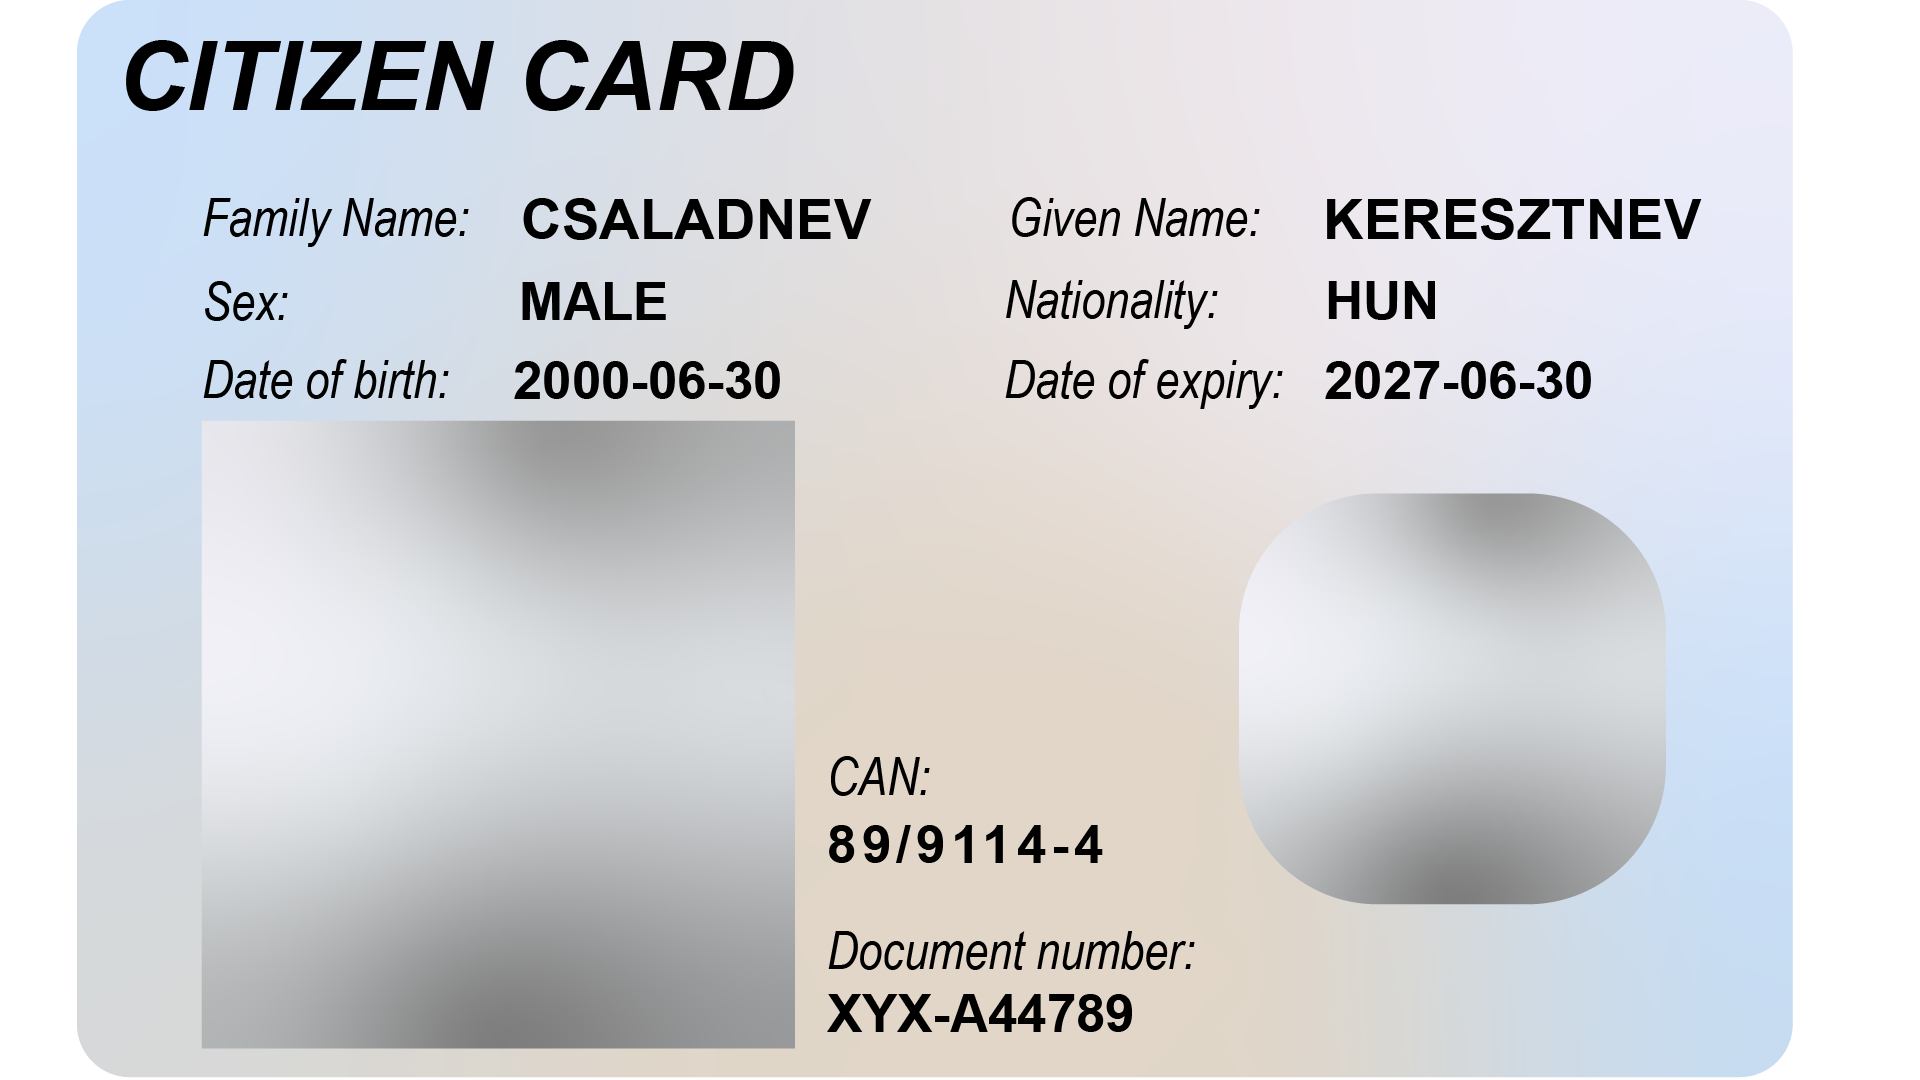
\includegraphics[scale=.2]{example_id_card_3.eps}}
    \caption{A harmadik példa igazolvány}
\end{figure}

A program futtatása során generált kép, és a az eredményt tartalmazó csv fájlt is igazolja a program helyes működését, ezzel az elrendezéssel is sikeres volt a szöveg kinyerés és feldolgozás.

\begin{tcolorbox}
    \begin{center}
        \begin{tabular}{ c c }
            CITIZEN CARD & N/A \\ 
            Family Name & CSALADNEV \\ 
            Given Name & KERESZTNEV \\ 
            Sex & MALE \\ 
            Nationality & HUN \\ 
            Date of birth & 2000-06-30 \\ 
            Date of expiry & 2027-06-30 \\ 
            CAN & 89/9114-4 \\ 
            Document number & XYX-A44789 \\ 
        \end{tabular}
    \end{center}
\end{tcolorbox}

\section{Az alkalmazás felépítése}

Strukturálisan az alkalmazás három fő egységre bontható. Az elsőbe sorolható minden olyan folyamat, amely a kép alapú dokumentumról való szövegkinyeréssel kapcsolatos. Ennek a folyamatnak az elején csupán egy fájl áll rendelkezésre, a végére viszont valamennyire rendezett formában, digitális formában már rendelkezünk a dokumentumról kinyert szövegről.
A második egységben ezen az adathalmazon elindulva először az osztálypéldányok létrehozása, feltöltése, és azok listába rendezése zajlik. Ez a lista lesz az, amin már el tud indulni a kulcs-érték párok keresésére írt algoritmus, melynek kimenete az a rendezett adathalmaz, amely a már egyéb lépések nélkül is helyes eredményt tartalmazza.
Mégis szükség van utófeldolgozásra, ez a harmadik egység. Az utófeldolgozás célja, hogy a felesleges, idő közben fontosságukat elveszített adatokat ne vigyük magunkkal tovább, többek között ilyenek például a koordináta adatok. Ez a lépés egy dictionary adatszerkezetbe rendezi az összes szöveget a párjával (ha van), így válik az adathalmazunk teljesen rendezetté. Ezután a szebb kimenet érdekében a szöveg formázása történik, ahol a felesleges karakterek és szóközök eltávolításra kerülnek.
Ezután az adathalmaz készen áll az exportálásra, melyet a program .csv kiterjesztéssel fog elmenteni.

\begin{figure}[h]
    \centerline{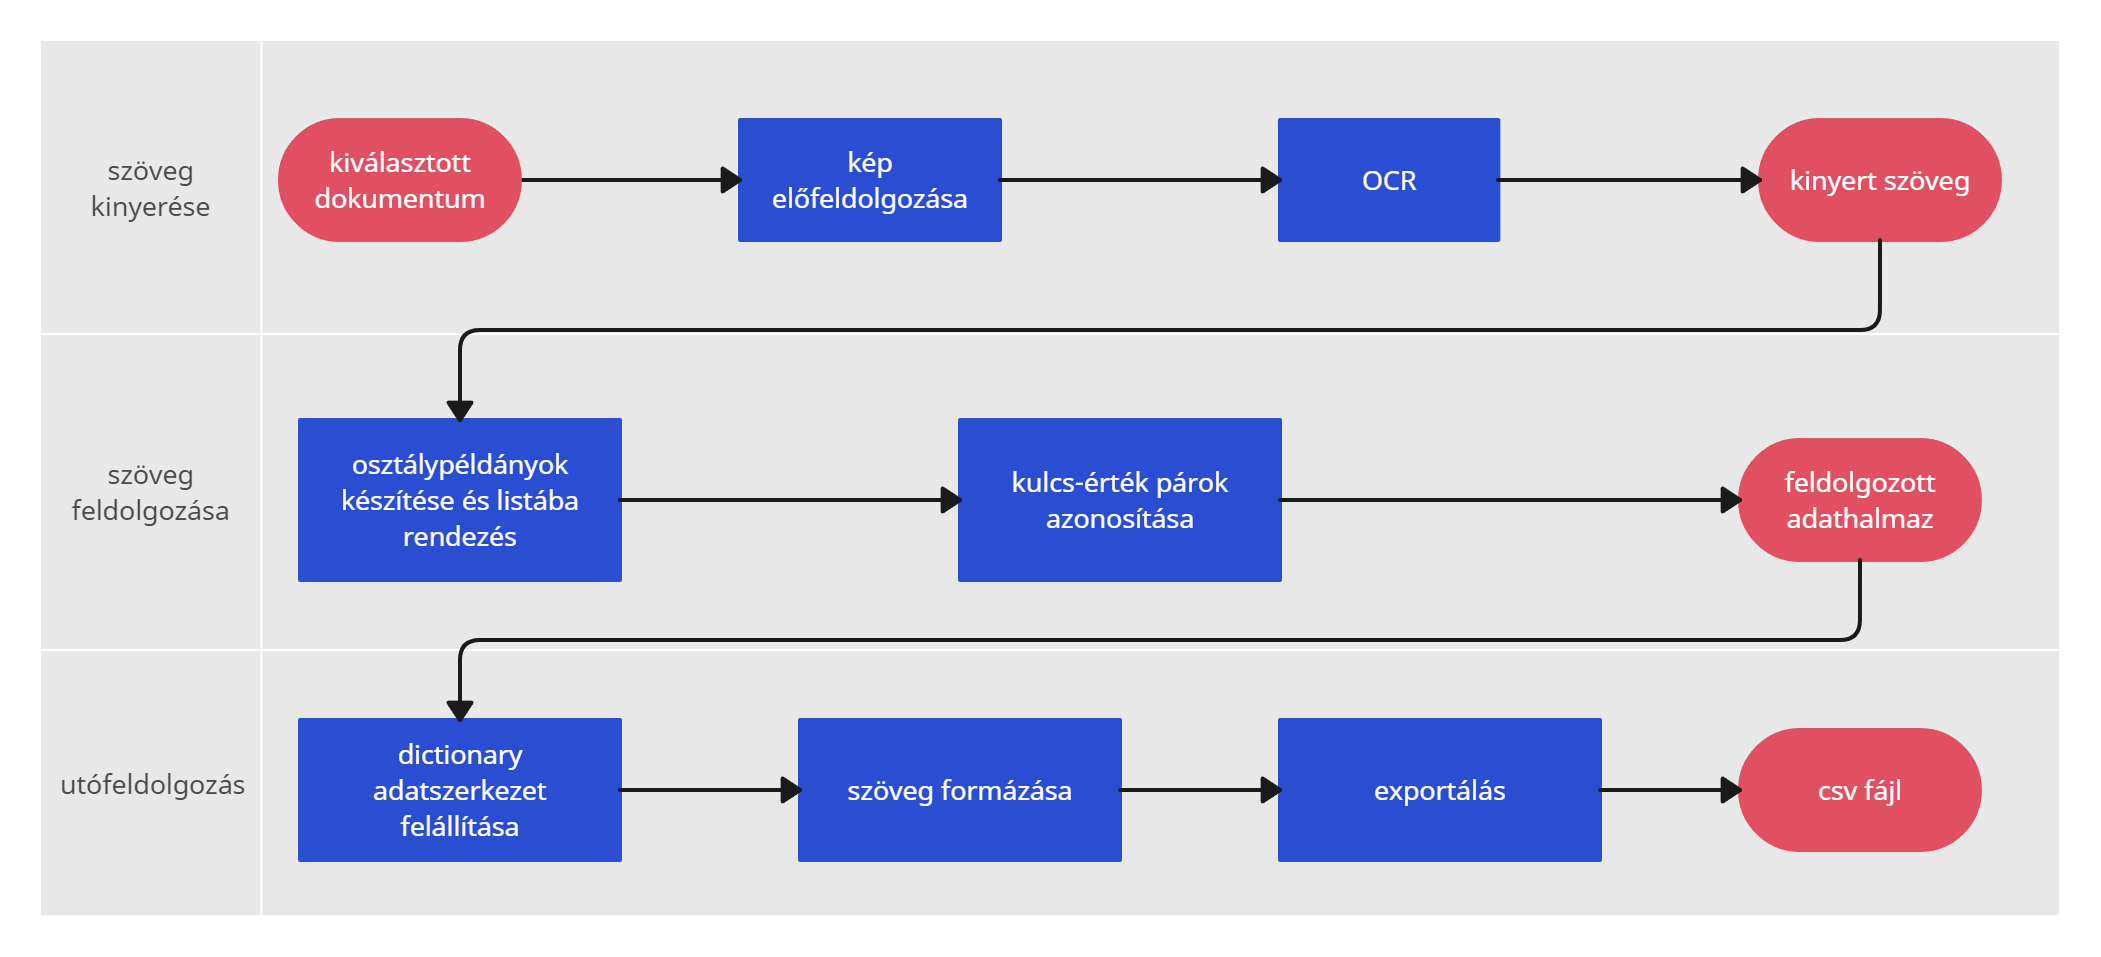
\includegraphics[scale=.21]{flowchart.eps}}
    \caption{Folyamatábra a program főbb lépéseiről}
\end{figure}

\section{Továbbfejlesztési lehetőségek}

A program számos ponton bővíthető új funkciókkal és beállítási lehetőségekkel. Az egyik legnagyobb értéket, de nem a legtöbb fejlesztés igénylő plusz beállítás a kimeneti fájl kiterjesztése lehetne. Előfordulhat olyan use-case, amikor nem csv kiterjesztésben szeretné a felhasználó az eredményt megkapni. Ez egy egyszerű legördülő menűből válaszható lenne, viszont mindegyik támogatott kiterjesztésnek saját export metódust kellene implementálni.
Nagyobb fejlesztést igényelne, de rendkívül hasznos lenne, hogyha egyszerre nem csak egy, hanem több kép alapú dokumentum is kiválasztható lenne. Ebben az esetben minden dokumentum kapna egy külön fájl, melyben a kinyert és párosított adatok találhatóak, de az mégjobb lenne, ha az azonos kulcsokat tartalmazó dokumentumok adatai egy fájlba kerülnének írásra, úgy, hogy a kulcsok csak egyszer szerepelnének, mint oszlopnév, és alattuk az összes, adott kulcshoz kinyert adat a dokumentumokról.
A felhasználó élményt javítaná, ha a tallózott dokumentum (vagy dokumentumok) előnézete látszódna a felületen, valamint ha az eredeti képen megjelenő, színes kerettel ellátott kép is az alkalmazáson belül jelenne meg, a jelenleg felugró ablak helyett. A beállítások halmaza bővíthető lenne még azzal is, hogy a program futásának eredménye a fájlba íráson túl akár azonnal kimásolható legyen egy szövegmezőből.

A kulcs-érték párokat kereső algoritmusban még rejtőzik potenciál. Jelenleg erősen korlátozott, hiszen a kulcshoz kapcsolódó érték keresése minden esetben először jobbra, majd lefelé történik a koordináta rendszerben. Például egy igazolványképen, ahol olyan táblázatos elrendezés van, melyen a kulcsok az értékek felett helyezkendnek el, és a kulcstól jobbra egy másik kulcs áll, mely alatt a hozzá tartozó érték, az algoritmus jelen állapotában ezt helytelenül értékelné ki. Ezt a limitációt lehetne csökkenteni, ha egyszerre vizsgálna mindkét irányba, és a környező elemeket is vizsgálva el tudná dönteni, hogy pontosan melyik érték tartozik hozzá. A vizsgálatba bele lehetne vonni az objektumok közötti távolságot is, mint heurisztika.
Ez egyfajta mesterséges intelligencia bevezetése lenne, hiszen a környező objektumok helyzetét elemezve és értékelve hozna döntést, és ez a döntés hatással lenne a következő kulcs érték keresésére is.

\chapter*{Összefoglalás}

A szakdolgozat elsődleges célja a szövegfeldolgozás témájának körbejárása volt egy olyan alkalmazás elkészítésével, mely az OCR technológiára alapozva képes igazolványokról készített képről szöveget kinyerni, majd ezeket egy saját algoritmus segítségével feldolgozni. A szakdolgozat segítségével betekintést nyerhettem a szövegfeldolgozás és karakterfelimserés világába, ám a kutató és fejlesztő munkák során megismertem számos egyéb képfeldolgozással kapcsolatos technológiát is. A program írása során törekedtem az egyetemen tanult fejlesztési módszerek használatára, és a szkriptnyelvek nevű kurzuson tanult Python tudásom kamatoztatására.
A modern fejlesztési irányelvek betartására is figyelemmel voltam, ezért használtam objektum orientáltságot is, a projekt komponenseinek átláthatóságáról pedig a programfájlok megfelelő szintű struktúráltsága gondoskodik.


\begin{thebibliography}{99}
\addtocontents{toc}{\ }
\addcontentsline{toc}{section}{Irodalomjegyzék}
\fontsize{10pt}{12pt}\selectfont

\bibitem{onlineocr}
Image to Text Converter

\emph{https://www.imagetotext.info/}
(Utolsó megtekintés: 2023.04.23)


\bibitem{ocr}
What Is Optical Character Recognition (OCR)?

\emph{https://www.ibm.com/cloud/blog/optical-character-recognition}

(Utolsó megtekintés: 2023.04.23)


\bibitem{ocr_aws}
How does OCR work?

\emph{https://aws.amazon.com/what-is/ocr/}
(Utolsó megtekintés: 2023.04.23)


\bibitem{handwritten_ocr}
Field typing for improved recognition on heterogeneous handwritten forms

\emph{https://arxiv.org/pdf/1909.10120.pdf}
(Utolsó megtekintés: 2023.04.23)


\bibitem{ocr_accuracy}
What affects OCR accuracy and how to improve it?

\emph{https://www.docsumo.com/blog/ocr-accuracy}
(Utolsó megtekintés: 2023.04.23)


\bibitem{f1_score}
The F1 score

\emph{https://towardsdatascience.com/the-f1-score-bec2bbc38aa6}

(Utolsó megtekintés: 2023.04.23)


\bibitem{imporve_accuracy}
Improve OCR Accuracy With Advanced Image Preprocessing

\emph{https://docparser.com/blog/improve-ocr-accuracy/}

(Utolsó megtekintés: 2023.04.23)


\bibitem{python}
Applications for Python

\emph{https://www.python.org/about/apps/}
(Utolsó megtekintés: 2023.04.23)


\bibitem{pytesseract2}
pytesseract 0.3.10

\emph{https://pypi.org/project/pytesseract/}
(Utolsó megtekintés: 2023.04.23)


\bibitem{pytesseract}
How to OCR with Tesseract, OpenCV and Python

\emph{https://nanonets.com/blog/ocr-with-tesseract/}
(Utolsó megtekintés: 2023.04.23)


\bibitem{easyocr}
EasyOCR on GitHub

\emph{https://github.com/JaidedAI/EasyOCR}
(Utolsó megtekintés: 2023.04.23)


\bibitem{opencv}
opencv-python 4.7.0.72

\emph{https://pypi.org/project/opencv-python/}
(Utolsó megtekintés: 2023.04.23)


\bibitem{opencv_functions}
Image Processing in OpenCV

\emph{https://docs.opencv.org/4.x/d2/d96/tutorial\_py\_table\_of\_contents\_imgproc.html}

(Utolsó megtekintés: 2023.04.23)


\bibitem{opencv_threshold}
Threshold Types in OpenCV

\emph{https://docs.opencv.org/4.x/d7/d1b/group\_\_imgproc\_\_misc.html}

(Utolsó megtekintés: 2023.04.23)


\bibitem{date_regex}
Sample regular expressions

\emph{https://docs.opswat.com/mdcore/proactive-dlp/sample-regular-expressions}

(Utolsó megtekintés: 2023.04.23)


\bibitem{country_codes}
Country Codes ALPHA-2 & ALPHA-3

\emph{https://www.iban.com/country-codes}
(Utolsó megtekintés: 2023.04.23)


\bibitem{tcl}
Tcl (Tool Command Language)

\emph{https://www.tcl.tk/}
(Utolsó megtekintés: 2023.04.23)


\bibitem{customtkinter}
CustomTkinter on GitHub

\emph{https://github.com/TomSchimansky/CustomTkinter}
(Utolsó megtekintés: 2023.04.23)


\end{thebibliography}


\chapter*{Nyilatkozat}
% \addtocontents{toc}{\ }
\addcontentsline{toc}{section}{Nyilatkozat}

\noindent
Alulírott Marosi Márk Dániel gazdaságinformatikus BSc szakos hallgató, kijelentem, hogy a dolgozatomat a Szegedi Tudományegyetem, Informatikai Intézet Szoftverfejlesztés Tanszékén készítettem, gazdaságinformatikus BSc diploma megszerzése érdekében. \hfill \break


\noindent
Kijelentem, hogy a dolgozatot más szakon korábban nem védtem meg, saját munkám eredménye, és csak a hivatkozott forrásokat (szakirodalom, eszközök, stb.) használtam fel. \hfill \break

\noindent
Tudomásul veszem, hogy szakdolgozatomat a Szegedi Tudományegyetem Diplomamunka Repozitóriumában tárolja.

\vspace*{2cm}


\begin{tabular}{lc}
Szeged, \today\
\hspace{2cm} & \makebox[6cm]{\dotfill} \\
& aláíras \\
\end{tabular}


\chapter*{Köszönetnyilvánítás}
\addcontentsline{toc}{section}{Köszönetnyilvánítás}

Ezúton szeretnék köszönetet mondani Janurik Viktor Bálint témavezetőmnek, aki lehetővé tette a dolgozat elkészülését. Nagyra értékelem a türelmét és megértését, ami hozzájárult az eredmények eléréséhez. \\

\noindent
Köszönet illeti azokat az oktatókat, tanárokat és szakembereket is, akik tanítottak és inspiráltak az egyetemi éveim során. Az általuk átadott tudás és tapasztalat nemcsak a szakdolgozatban, hanem az életemben is hasznos lesz. \\

\noindent
Nem utolsó sorban köszönetet szeretnék mondani Gyikó Richárd külső témavezetőmnek is, aki szakmai hozzáértésével, támogatásával és iránymutatásával járult hozzá a szakdolgozat elkészüléséhez.

\end{document}